\chapter{Construction: Iterations}
\label{chap:construction}

\section*{Introduction}
\addcontentsline{toc}{section}{Introduction}

This chapter presents the construction phase, during which CANvisionNative was built on the architecture baseline of Chapter~\ref{chap:elaboration}. It first explains how the work of the phase was planned in iterations, then presents the four iterations one after the other: the first detection pipeline and client, its validation and correction on a real recording, the hardware layer and its bench rig, and the rebuild of the vehicle models.

\section{Iteration planning}
\label{sec:it-planning}

The construction phase was divided into four iterations, each one addressing some of the risks of Table~\ref{tab:risks}. Each iteration is presented with the same template: its objectives, the use cases it addressed, its design, its implementation, its tests, and an assessment that decided what the next iteration had to do. Table~\ref{tab:iterations} gives the period, the goal and the main risks addressed by each iteration.

\begin{table}[H]
\centering
\small
\caption{Iterations of the construction phase.}
\label{tab:iterations}
\begin{tabularx}{\textwidth}{|P{1.8cm}|P{2.2cm}|Y|P{3.4cm}|}
\hline
\textbf{Iteration} & \textbf{Period (2026)} & \textbf{Goal} & \textbf{Main risks addressed} \\
\hline
1 & March to June & First detection pipeline and client (M3 to M8) & R2, R7 \\
\hline
2 & June to July & Validation and correction on a Kia EV6 recording & R3, R6, R7, R8 \\
\hline
3 & August to September & Hardware layer and bench rig (M2) & R1 \\
\hline
4 & September & Model rebuild and evaluation on recordings kept out of training & R3, R4, R5, R6 \\
\hline
\end{tabularx}
\end{table}

% ============================================================
\section{Iteration 1: first detection pipeline and client}
\label{sec:it1}

\subsection{Objectives}

The first iteration delivered milestones M3 to M8 on the architecture baseline: models trained for several vehicles and driving states (M3), the explanation engine (M4), the real time charts (M5), session recording (M6), the integration of the client and the backend (M7), and the decoding pipeline for offline and live traffic (M8). At its end, an analyst could import a log, analyse and replay it, review and explain its alerts, and export them.

\subsection{Use cases addressed}

This iteration addressed the use cases \emph{Import log}, \emph{Select vehicle}, \emph{Replay log}, \emph{Start live simulation}, \emph{Detect anomaly}, \emph{Record session}, \emph{Review alerts}, \emph{Request explanation}, \emph{Export report} and \emph{Configure settings}, which together cover the work of the analyst on a recorded log. The use cases \emph{Connect hardware}, \emph{Check model status} and \emph{Describe capture} were addressed in later iterations.

\subsection{Design: a first model based on driving states}
\label{sec:impl-state}

The first design routed each frame through a driving state. Fourteen rolling features were computed for every identifier, a K-Means model shared by all vehicles classified the state as parking, idle or driving (Figure~\ref{fig:state-vehicle}), and the frame was scored by the Isolation Forest of that state and vehicle. When no forest matched, the engine fell back to a generic model, then to a heuristic. These models were trained on more than seven million frames from sixty six sources of the corpus of Table~\ref{tab:datasets}.

\begin{figure}[H]
\centering
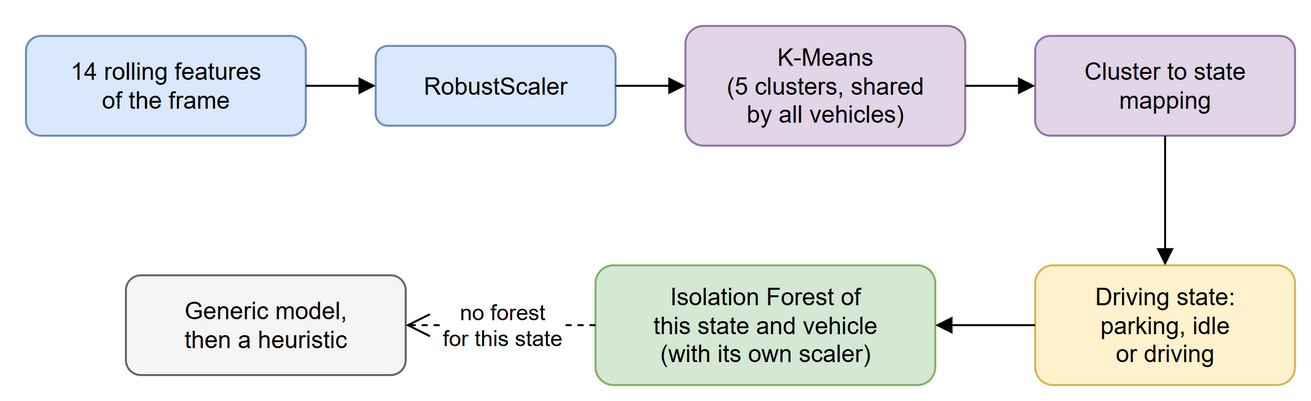
\includegraphics[width=\textwidth]{state_vehicle.png}
\caption[Scoring path of the first design.]{Scoring path of the first design: K-Means on fourteen rolling features chose the driving state, which selected the Isolation Forest.}
\label{fig:state-vehicle}
\end{figure}

\subsection{Implementation}

The iteration implemented the backend services below on the architecture baseline, then the screens and exports of the client.

\subsubsection{Parser and common frame representation}
\label{sec:impl-parser}

One dispatch function turns every supported format into the same stream of (timestamp, identifier, payload) frames:

\begin{itemize}
    \item \textbf{.csv:} Generic columns, or the SavvyCAN columns with timestamps in microseconds.
    \item \textbf{.mf4:} ASAM \gls{mf4}~\cite{asam_mdf} binary logs, read with asammdf.
    \item \textbf{.asc:} The Vector text format.
    \item \textbf{.log:} The candump and SocketCAN format, including its timestamped variant.
    \item \textbf{.txt:} The PCAN text format, with candump parsing as a fallback.
\end{itemize}

The offline analysis called this function from the start. The replay engine, however, still had its own loader, which only understood \gls{csv}; this gap was found and closed in the second iteration (Fix 4).

\subsubsection{Replay engine}
\label{sec:impl-replay}

The replay process writes partial results during the run, so that the client can show progress, and a summary with the full alert list at the end. In the client, the Log Playback screen plays the frames at the pace of their own timestamps, multiplied by the chosen speed; a first version played one frame per screen refresh, which ran a bus of 3{,}000 frames per second about fifty times slower than real time.

\Needspace{335pt}% keep the heading with its float
\subsubsection{Vehicle profiles}
\label{sec:impl-vehicle}

Two registries describe the vehicles. The vehicle profiles (Table~\ref{tab:vehicles}) give a bitrate and the \gls{dbc} files that decode the frames; the last one was written for the bench rig in the third iteration. The second registry lists the trained models of each vehicle. The two lists do not match one to one: the Jaguar I-PACE has a model but no \gls{dbc} file, while the BMW i3 has a \gls{dbc} file but only a model of the first design.

\begin{table}[H]
\centering
\small
\caption{Vehicle profiles with \acrshort{dbc} decoding.}
\label{tab:vehicles}
\begin{tabular}{|l|l|c|}
\hline
\textbf{Identifier} & \textbf{Display name} & \textbf{Bitrate} \\
\hline
nissan\_leaf    & Nissan Leaf (2019, 40/62 kWh) & 500 kbps \\
\hline
hyundai\_ioniq5 & Hyundai Ioniq 5               & 500 kbps \\
\hline
hyundai\_kia    & Hyundai / Kia (generic)       & 500 kbps \\
\hline
skoda\_enyaq    & Škoda Enyaq iV (VW MEB)       & 500 kbps \\
\hline
vw\_skoda\_audi & VW / Škoda / Audi (generic)   & 500 kbps \\
\hline
renault\_zoe    & Renault Zoe                   & 500 kbps \\
\hline
tesla\_model3   & Tesla Model 3                 & 500 kbps \\
\hline
kia\_ev6        & Kia EV6                       & 500 kbps \\
\hline
bmw\_i3         & BMW i3 (2017, 60 Ah REX)      & 500 kbps \\
\hline
bench\_rig      & Arduino bench rig             & 500 kbps \\
\hline
\end{tabular}
\end{table}

\subsubsection{Explanation module}

The explanation module implements the design of \Sref{sec:design-ai}. The context of an alert is built in the backend, and the providers are called in turn through their \gls{http} interfaces. Each explanation is added to a history store, so that later similar anomalies can refer to it, and cached during a run, so that the same alert is not explained twice.

\subsubsection{Client and exports}

The client implements the seven screens of \Sref{sec:design-frontend}, presented in Chapter~\ref{chap:transition}. Anomaly Intel exports the alert list as a \gls{csv} file or as a PDF report built with PDFsharp, both read from the list on screen.

\subsection{Tests}

Each milestone was checked by running it on recorded logs and by a demonstration in the client before the next one started. The systematic validation of the whole pipeline on a real recording was left to the second iteration.

\subsection{Assessment}

All the milestones M3 to M8 were delivered, and the first pipeline worked from the import of a log to the export of its alerts. It had not yet been checked against facts known independently, which was the goal of the second iteration.

% ============================================================
\section{Iteration 2: validation and correction on the Kia EV6}
\label{sec:it2}

\subsection{Objectives}

The second iteration validated the first pipeline on a real recording, found its defects and corrected them. One rule guided it (NFR2): a claim had to be backed by reproducible evidence before any code was changed. Tuning a threshold or retraining blindly were not accepted as fixes. A defect counted as found only once it could be triggered on demand and explained in the code, and as fixed only once the same test, run again, gave the expected result.

\subsection{Use cases addressed}

The validation followed the path of an analyst on a recording, through the use cases \emph{Import log}, \emph{Select vehicle}, \emph{Replay log} and \emph{Detect anomaly}, then \emph{Request explanation} and \emph{Export report} on the alerts that the replay produced.

\Needspace{388pt}% keep the text with its float
\Needspace{374pt}% keep the heading with its float
\subsection{Design of the validation}

The validation took three passes (Figure~\ref{fig:validation-workflow}): an audit of the interface, an analysis of the root causes of the alerts, and the correction of the defects, each verified again, followed by a full run of the corrected pipeline.

\begin{figure}[H]
\centering
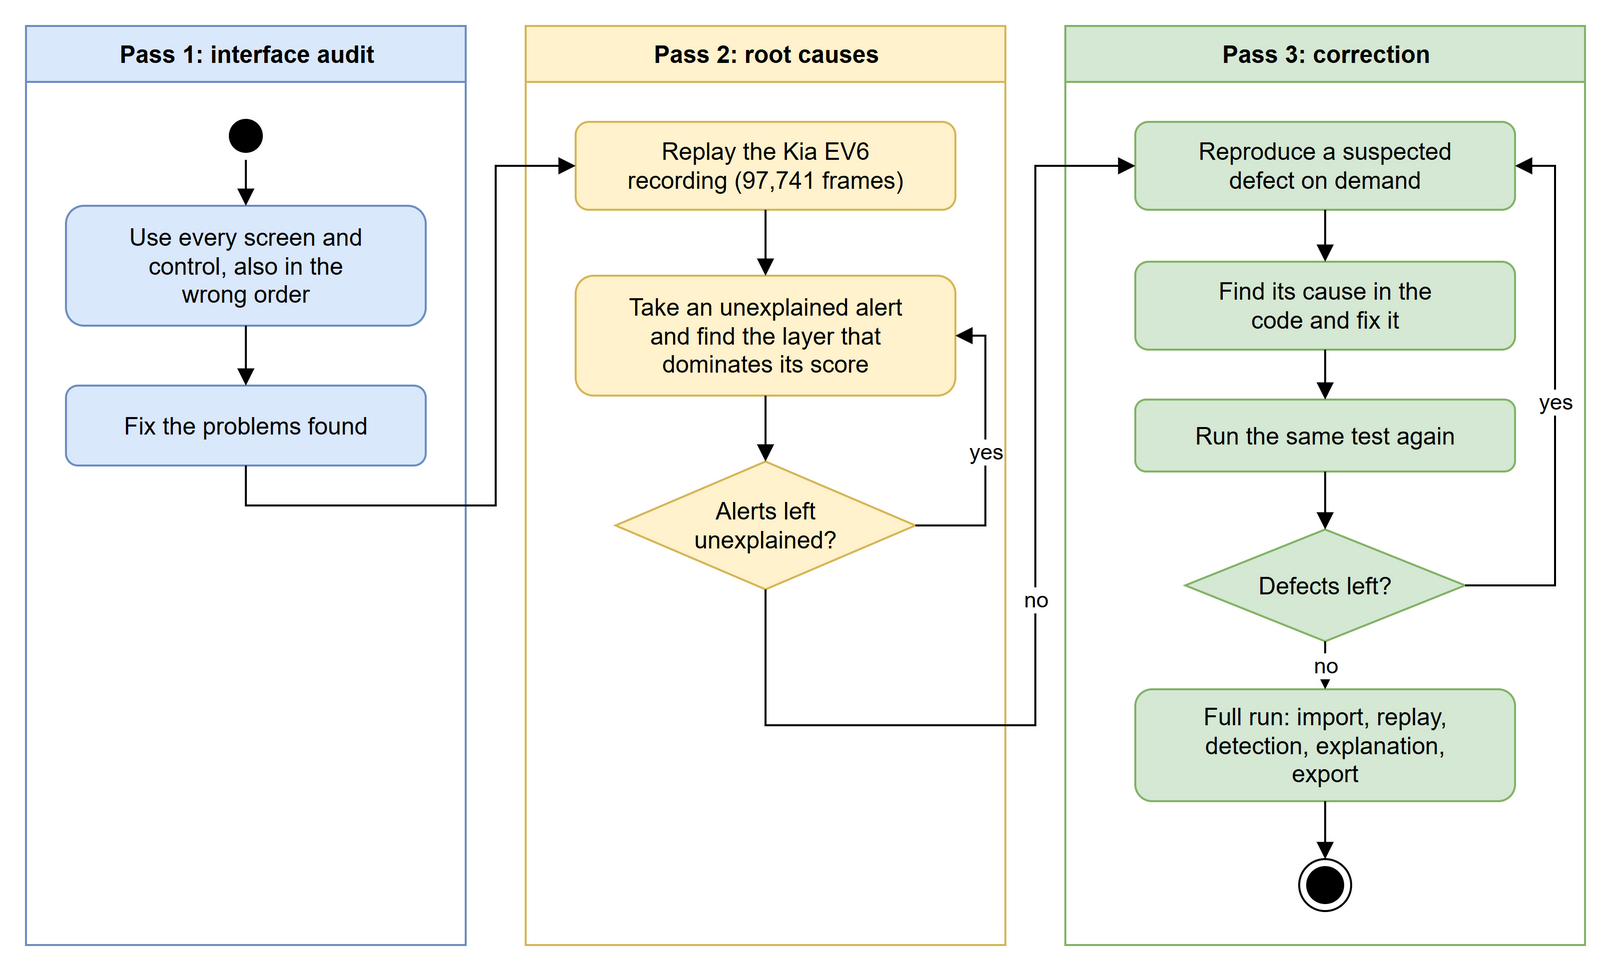
\includegraphics[width=0.9\textwidth]{validation_workflow.png}
\caption{Passes of the validation of the first pipeline.}
\label{fig:validation-workflow}
\end{figure}

\label{sec:validation-setup}
The iteration used a one hour recording of a Kia EV6 (\texttt{00000158-\allowbreak 64CBC290.MF4}) from the CSS Electronics EV Data Pack (Table~\ref{tab:datasets}), captured by a CANedge logger that actively polled the \glspl{ecu} with \gls{uds} requests. After conversion, it contains \textbf{97{,}741 frames}. It was the only available recording that came from an unmodified production vehicle, was long enough for measurements before and after a fix, had a frame count that could be checked against the metadata of the file, and belonged to a vehicle with its own profile and model. A candump log of a Renault Clio, from another vehicle and logger, served to check that no data leaks between sessions.

\subsection{Implementation: audit and corrections}

The iteration started with an audit of the interface, fixed the conversion of the recording, then analysed the alerts and corrected the defects they revealed.

\subsubsection{Interactive interface audit}

Before looking at the data, we drove the running client through interface automation: every screen, the import of valid, empty, corrupted and very large files, the full life cycle of a replay, and actions done in the wrong order or several times. This revealed an implausible latency shown on three screens, a rendering problem caused by a font substitution, and destructive actions that ran without confirmation, all fixed before the data driven validation.

\subsubsection{Conversion of the MF4 file}
\label{sec:impl-mf4}

Loggers of the CANedge type spread the traffic of an \gls{mf4} file over several channel groups, most of them empty templates. Our first conversion used the default view of the library, which shows only the first channel group and silently drops the others, so it returned a small part of the traffic. The conversion now goes through every group and merges those that hold data; checking the number of frames against the metadata of the file confirmed the fix and gave the 97{,}741 frames used in this iteration.

\subsubsection{Root cause analysis of the alerts}
\label{sec:validation-rootcause}

Before any correction, the replay produced \textbf{15{,}945 alerts}, an alert rate of 16.3\% that made the system hard to use. Instead of raising the threshold, we attributed every alert to the layer that dominated its score (Table~\ref{tab:rootcause}).

\begin{table}[H]
\centering
\caption{Root causes of the 15,945 alerts of the first pipeline.}
\label{tab:rootcause}
\begin{tabular}{|P{3.4cm}|r|P{7.5cm}|}
\hline
\textbf{Dominant cause} & \textbf{Share} & \textbf{Explanation} \\
\hline
Machine learning layer & 61.42\% & Wrong model selected, and wrong driving state (Fixes 1 and 2) \\
\hline
Timing layer & 31.51\% & Irregular intervals of the \gls{uds} polling, which gives a very high alert rate on the polled identifiers by construction \\
\hline
Payload layer & 7.07\% & Real variation of the sensor values in a battery telemetry message \\
\hline
\textbf{Total explained} & \textbf{100\%} & \\
\hline
\end{tabular}
\end{table}

The machine learning share pointed at the defects in model selection and state classification below; the timing and payload shares were explained by the \gls{uds} polling and by real sensor variation, so they were not treated as defects. Four defects came from this analysis, and two more appeared when the corrections were checked through the application rather than through the backend \gls{api} alone. Each is presented as problem, investigation, root cause, fix, evidence and result.

\subsubsection{Fix 1: vehicle model selection}

\begin{itemize}
    \item \textbf{Problem:} Choosing a vehicle in the client had no visible effect: every replay seemed to score the frames the same way.
    \item \textbf{Investigation:} We followed the vehicle identifier from the selector of the client, through the \gls{rest} call and the replay process, down to the scoring call.
    \item \textbf{Root cause:} The scoring step never received the vehicle chosen by the analyst. The replay engine created its scoring component without telling it which vehicle was active, so every replay was scored with the generic model.
    \item \textbf{Fix:} We passed the vehicle identifier through every stage that sets up scoring: the replay engine, the offline analysis, the live hardware interface, the backend endpoint and the whole call chain of the client down to the selector.
    \item \textbf{Evidence:} We read the command line of the replay process in the process list of the operating system and confirmed that it started with the chosen vehicle. We also confirmed that the vehicle list of the backend returned the same identifier as the folder of the trained model on disk.
    \item \textbf{Result:} Every replay now scores the frames with the model of the chosen vehicle, as required by FR2.
\end{itemize}

\subsubsection{Fix 2: driving state classification}
\label{sec:fix2}

\begin{itemize}
    \item \textbf{Problem:} The state classifier reported \textbf{99.93\%} of the recording (97{,}677 of 97{,}741 frames) as ``parking'', although the recording is an hour of active driving.
    \item \textbf{Investigation:} We compared, field by field, the feature vector and the scaling given to the classifier with the feature list and the scaler used to train the K-Means model.
    \item \textbf{Root cause:} Two defects added up. The vector given to the classifier was built from a list of 11 features meant for the scoring model, while the K-Means model had been trained on 14 features, so every call raised the error ``expected 14 features, got 11''. A very broad error handler caught this error and always returned ``parking'', which made the failure constant and therefore invisible unless someone reproduced the exact error on purpose.
    \item \textbf{Fix:} We corrected the feature list to the 14 features in the order used at training, and added the scaling step that was missing before the classification.
    \item \textbf{Evidence:} After the fix, the same recording was classified as \textbf{99.92\% ``driving''} (97{,}667 of 97{,}741 frames), with 64 frames ``unknown'' and 10 ``parking'', a credible result for an hour of driving.
    \item \textbf{Result:} The Isolation Forest of the right state is now used for almost every frame. This fix explains most of the improvements reported in \Sref{sec:validation-beforeafter}.
\end{itemize}

\subsubsection{Fix 3: attribution of the reason}

\begin{itemize}
    \item \textbf{Problem:} The layer shown to the analyst as the ``dominant'' cause of an alert did not match what the fused score had actually used.
    \item \textbf{Investigation:} We traced the displayed label back from the \gls{api} response to the internal reason string, and compared it with the real inputs of the fusion.
    \item \textbf{Root cause:} The label took the largest of all the values of the reason string, including two fields kept only for diagnosis: a raw frequency, sometimes in the thousands of hertz, and a raw entropy. These two values are much larger than the four real inputs of the fusion, so they almost always won and the displayed cause was wrong. The same mistake had been written independently six times in four files.
    \item \textbf{Fix:} We restricted the comparison, in all six places, to the four fields that really feed the fused score: timing, payload, machine learning and persistence.
    \item \textbf{Evidence:} By inspecting the inputs of the fusion component, we confirmed that it only uses the normalised layer scores, persistence being computed inside it. The wrong label had therefore never changed the detection itself, only its explanation. After the fix, the alert feed named the right layer, for example the payload layer when it really dominated.
    \item \textbf{Result:} The cause shown for an alert now matches the real inputs of its score everywhere, which makes both the alert list and the explanations built from it more trustworthy.
\end{itemize}

\subsubsection{Fix 4: one parser for replay}

\begin{itemize}
    \item \textbf{Problem:} Some formats that the file dialog accepted gave empty or meaningless replays.
    \item \textbf{Investigation:} We compared the loading code of the replay engine with the shared loader of \Sref{sec:impl-parser}, which the offline analysis already used without problems.
    \item \textbf{Root cause:} The replay engine had its own loading code, which called a generic \gls{csv} reader directly. Any .log, .asc or .txt file chosen in the dialog was read as a broken \gls{csv} file.
    \item \textbf{Fix:} The replay engine now calls the shared loader, and its own \gls{csv} only code was removed.
    \item \textbf{Evidence:} The corrected \gls{csv} path gave exactly the same output as before on all 97{,}741 frames, and small candump and Vector test files, which had produced timestamps and identifiers equal to zero, were parsed correctly.
    \item \textbf{Result:} Replay and offline analysis share one parsing path for every format, as required by NFR4.
\end{itemize}

\subsubsection{Fix 5: polling timer left stopped}

\begin{itemize}
    \item \textbf{Problem:} After a log had been imported from the Home screen, no later replay could deliver its alerts to the Anomaly Intel screen until the application was restarted.
    \item \textbf{Investigation:} The defect only appeared through the client, never through direct calls to the backend, which is why the backend tests behind Fixes 1 to 4 missed it and it only showed up during the end to end run.
    \item \textbf{Root cause:} Importing a log from the Home screen called a method that stopped the background polling timer of the client before its own analysis, and nothing started it again.
    \item \textbf{Fix:} The timer is now started again every time a replay is triggered, whatever the screen that triggered it.
    \item \textbf{Evidence:} A replay started after an import from the Home screen delivered its alerts to the Anomaly Intel screen again, like a replay started without a previous import.
    \item \textbf{Result:} Alerts now reach the analyst whatever the order of the screens used, a defect that a test of the backend alone could not have found.
\end{itemize}

\subsubsection{Fix 6: stale explanation cache}
\label{sec:validation-ai}

\begin{itemize}
    \item \textbf{Problem:} A request for the explanation of the alert displayed in the client could return the text of another, unrelated alert.
    \item \textbf{Investigation:} We replayed two datasets from different vehicles, the Kia EV6 recording and the Renault Clio log, one after the other, and compared the explanations returned for the same alert index in both runs.
    \item \textbf{Root cause:} The explanation endpoint looks up an alert index in a shared list that lives as long as the process. Before the fix, only the offline analysis and the injection of test anomalies filled this list, never a finished replay. An explanation could therefore be looked up in data left by an earlier analysis, or, before a replay finished, in data left by an even older session.
    \item \textbf{Fix:} Two changes closed the problem. When a replay finishes, its alerts are now published into the same shared list as the other two paths. When a replay starts, this list is cleared at once, so that nothing from a previous session can be found, even before the new replay ends.
    \item \textbf{Evidence:} For every alert index we checked, the explanation matched the identifier and the score of that alert in both datasets, with no trace of the other dataset. A second test filled the shared list with the Renault Clio data, started the Kia EV6 replay and asked for an explanation before the replay finished: the endpoint correctly returned no explanation instead of the old data.
    \item \textbf{Result:} An explanation now always belongs to the alert shown on screen, during and after a replay, which supports the trust required by NFR3.
\end{itemize}

\subsection{Tests: measurements before and after the corrections}
\label{sec:validation-beforeafter}

Table~\ref{tab:before-after} and Figure~\ref{fig:chart-before-after} compare the measurements on the same recording before any correction and after the four data driven fixes.

\begin{table}[H]
\centering
\caption{Before and after the corrections, on the Kia EV6 recording (97,741 frames).}
\label{tab:before-after}
\begin{tabular}{|l|r|r|}
\hline
\textbf{Metric} & \textbf{Before} & \textbf{After} \\
\hline
Total alerts & 15{,}945 (16.3\%) & 11{,}971 (12.25\%) \\
\hline
Replay duration & 685 s & 502.2 s \\
\hline
Throughput & about 143 frames/s & about 194.6 frames/s \\
\hline
Driving state & 99.93\% parking & 99.92\% driving \\
\hline
Saturated machine learning score ($\geq$ 0.999) & 77.6\% to 78.6\% & 0.0\% \\
\hline
\end{tabular}
\end{table}

\begin{figure}[H]
\centering
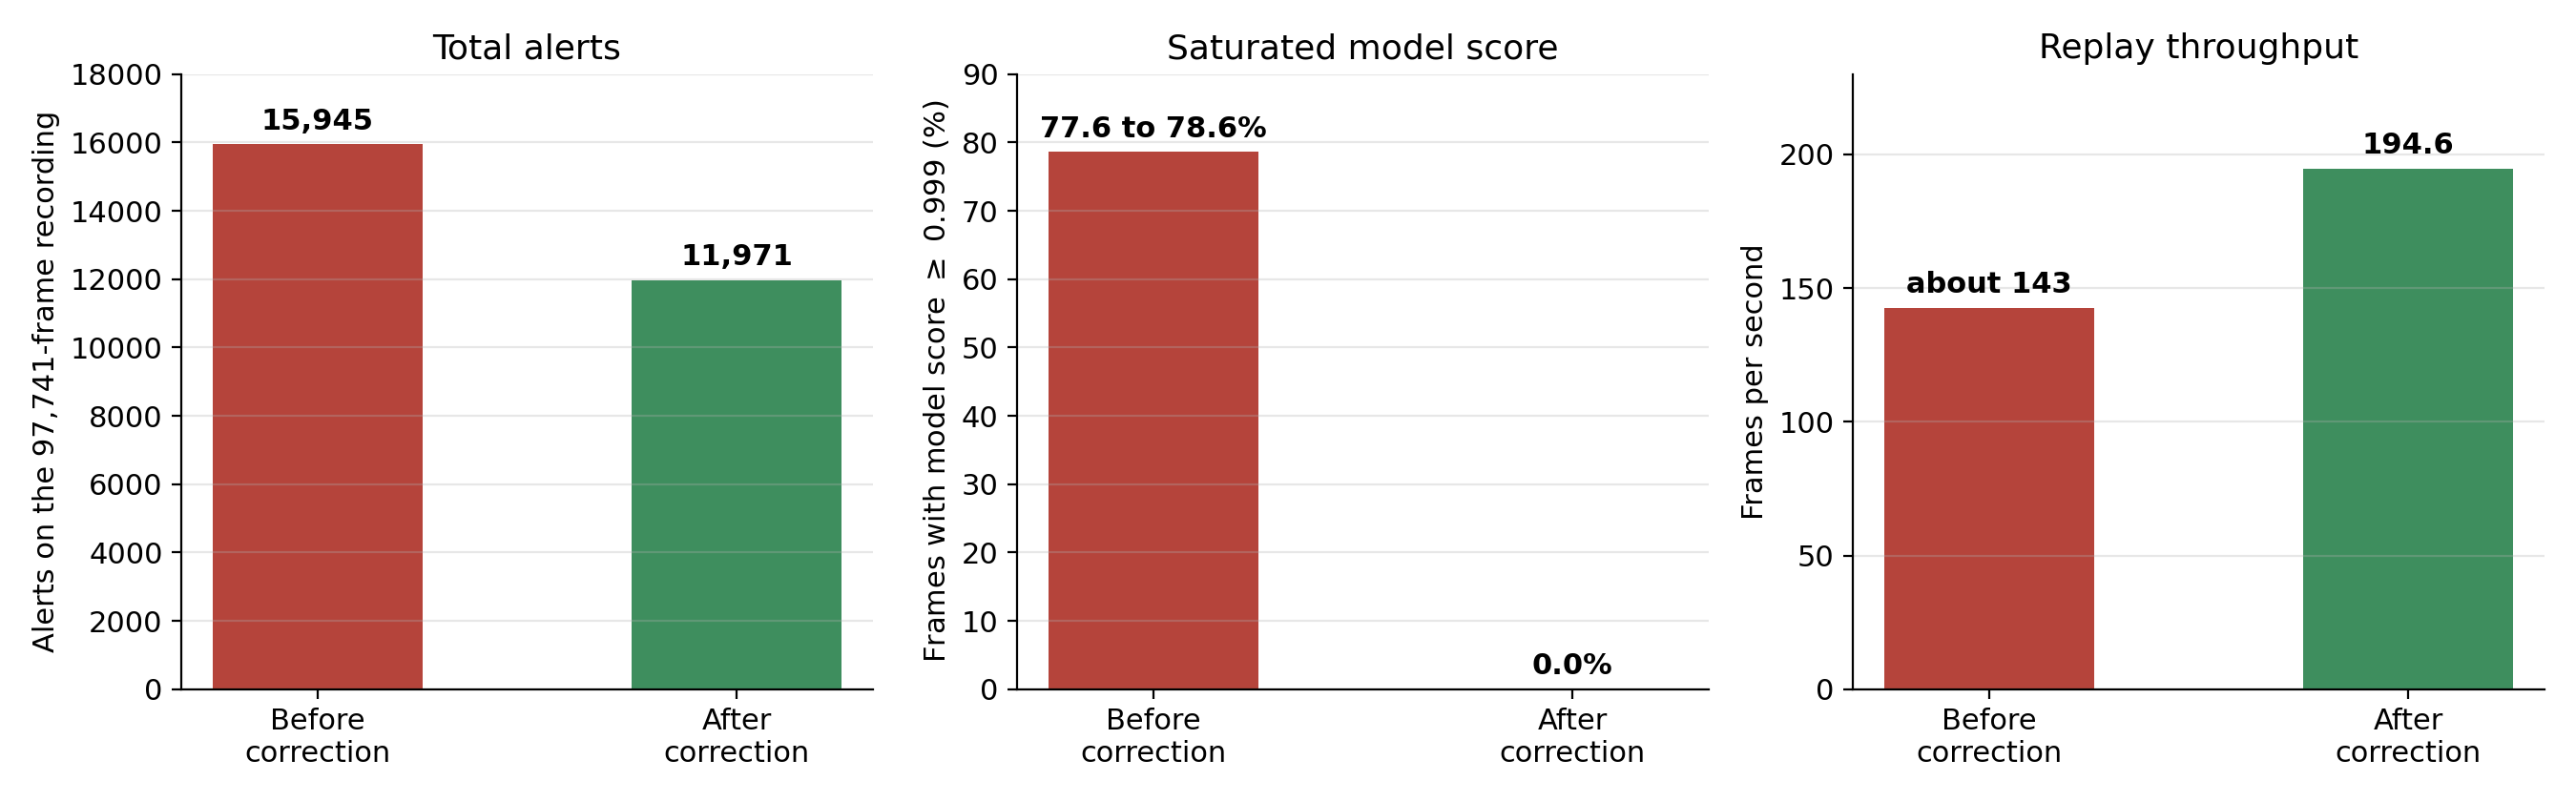
\includegraphics[width=\textwidth]{before_after_summary.png}
\caption{Alerts, saturated model score and replay throughput on the Kia EV6 recording, before and after the corrections.}
\label{fig:chart-before-after}
\end{figure}

\Needspace{278pt}% keep the text with its float
Fewer alerts and a higher throughput are side effects of fixing real defects, not of a threshold change: the right model of the vehicle replaced a saturated generic path. Figure~\ref{fig:chart-state} shows the evidence of Fix 2.

\begin{figure}[H]
\centering
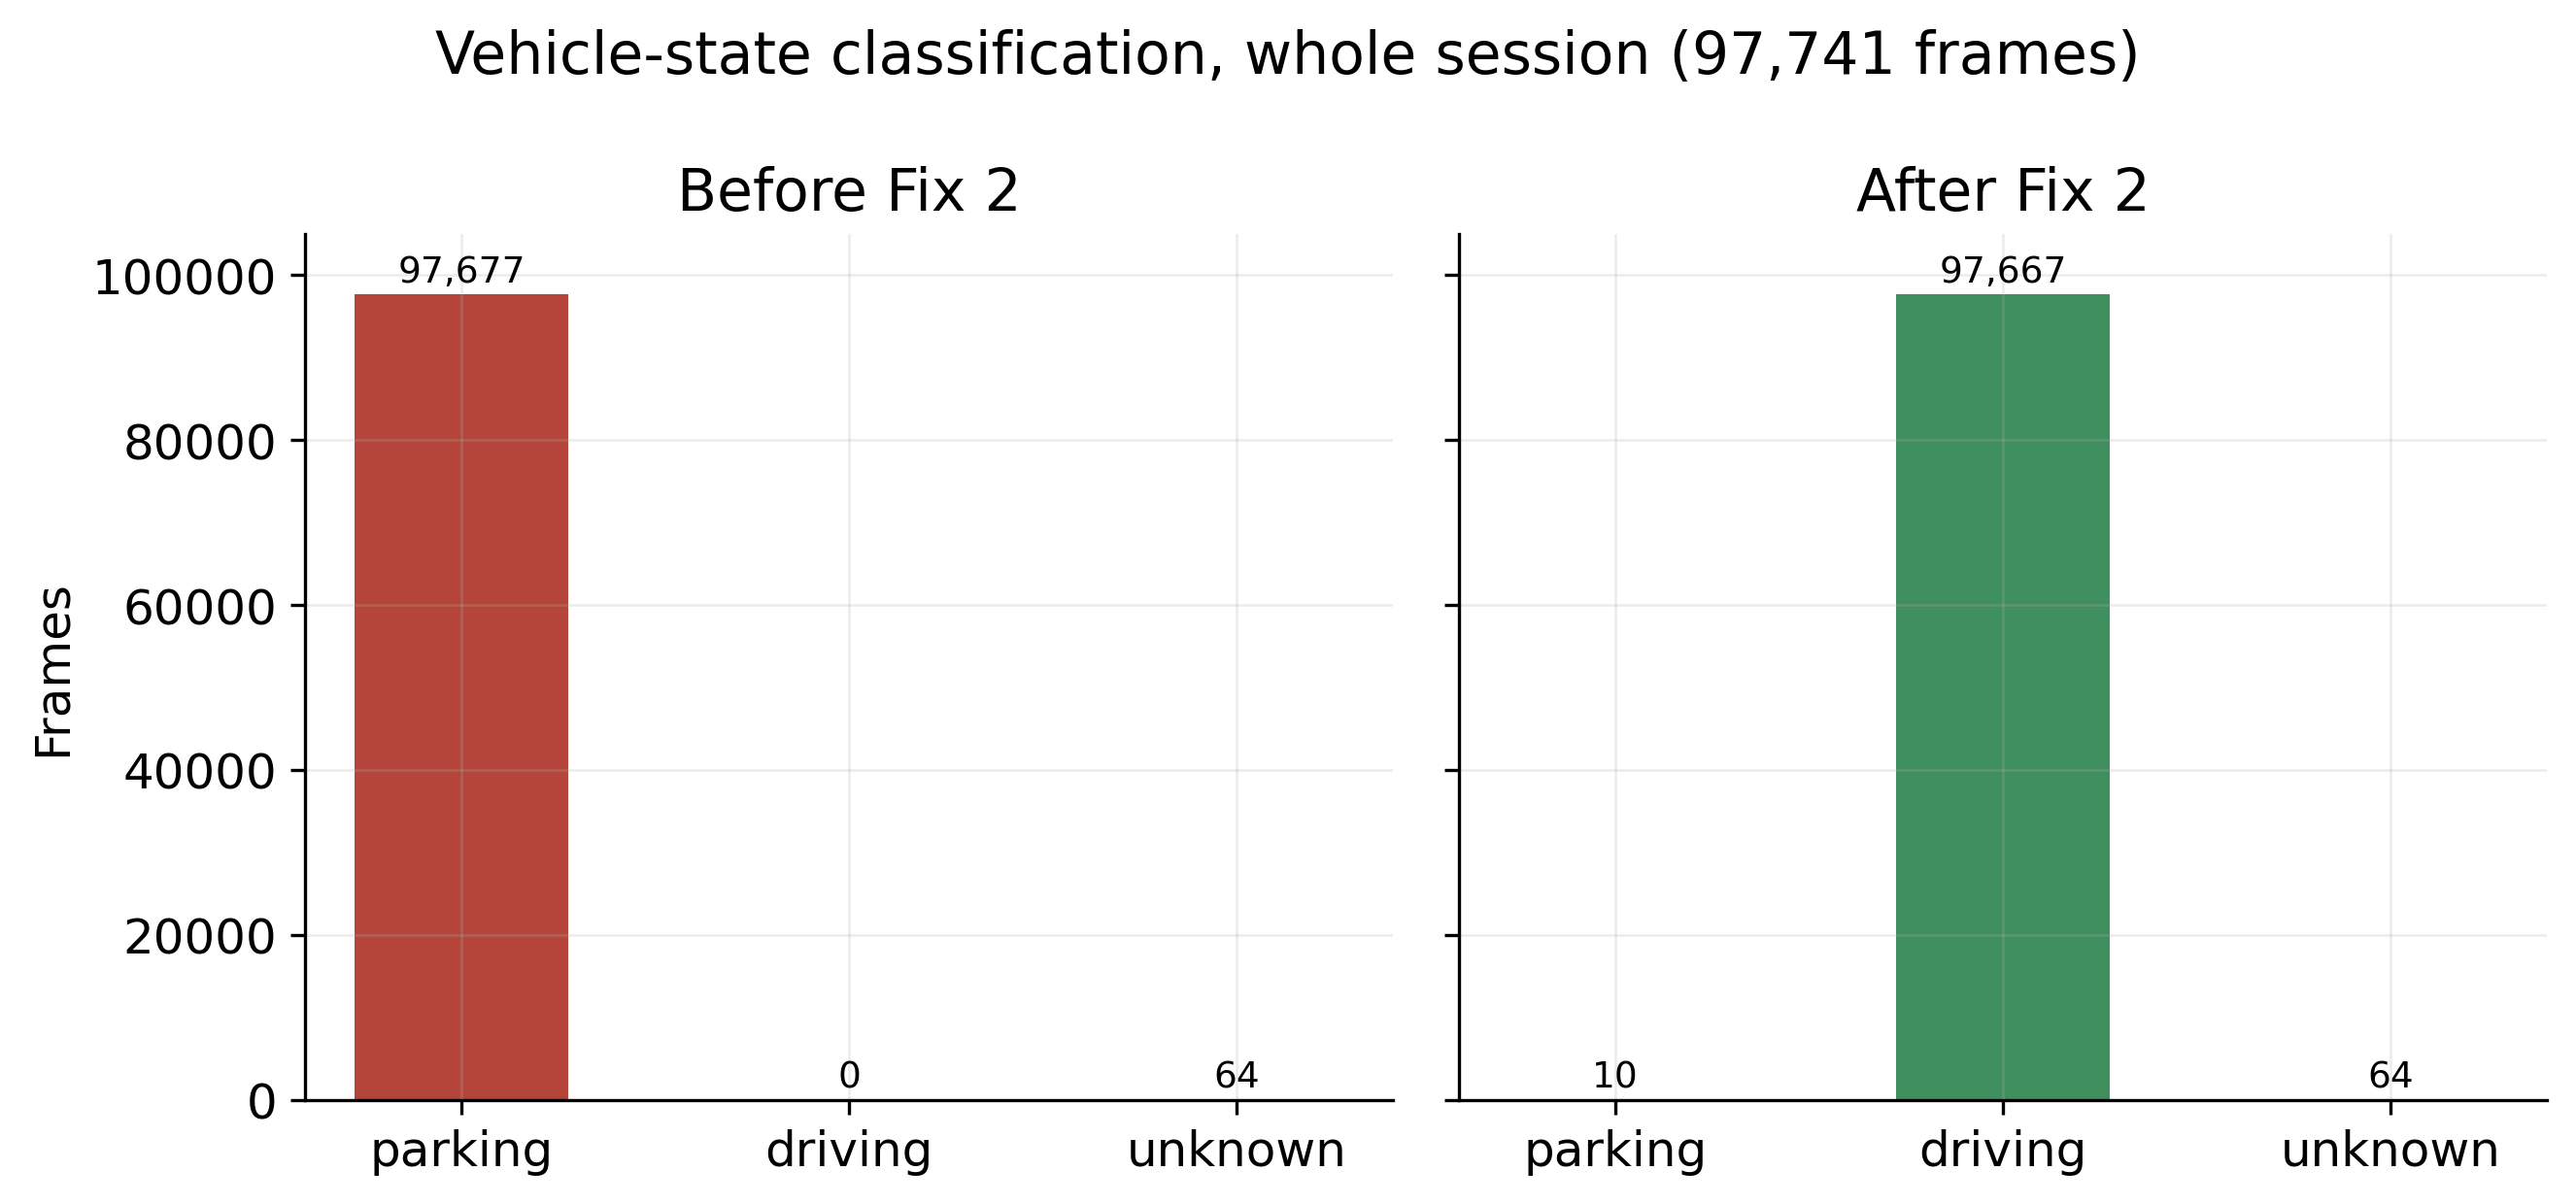
\includegraphics[width=0.85\textwidth]{state_classification_before_after.png}
\caption{Driving state of the whole recording, before and after Fix 2.}
\label{fig:chart-state}
\end{figure}

Figure~\ref{fig:chart-severity} breaks down the 11{,}971 remaining alerts. The right chart also supports Fix 3: the raw frequency and entropy no longer appear among the dominant layers.

\begin{figure}[H]
\centering
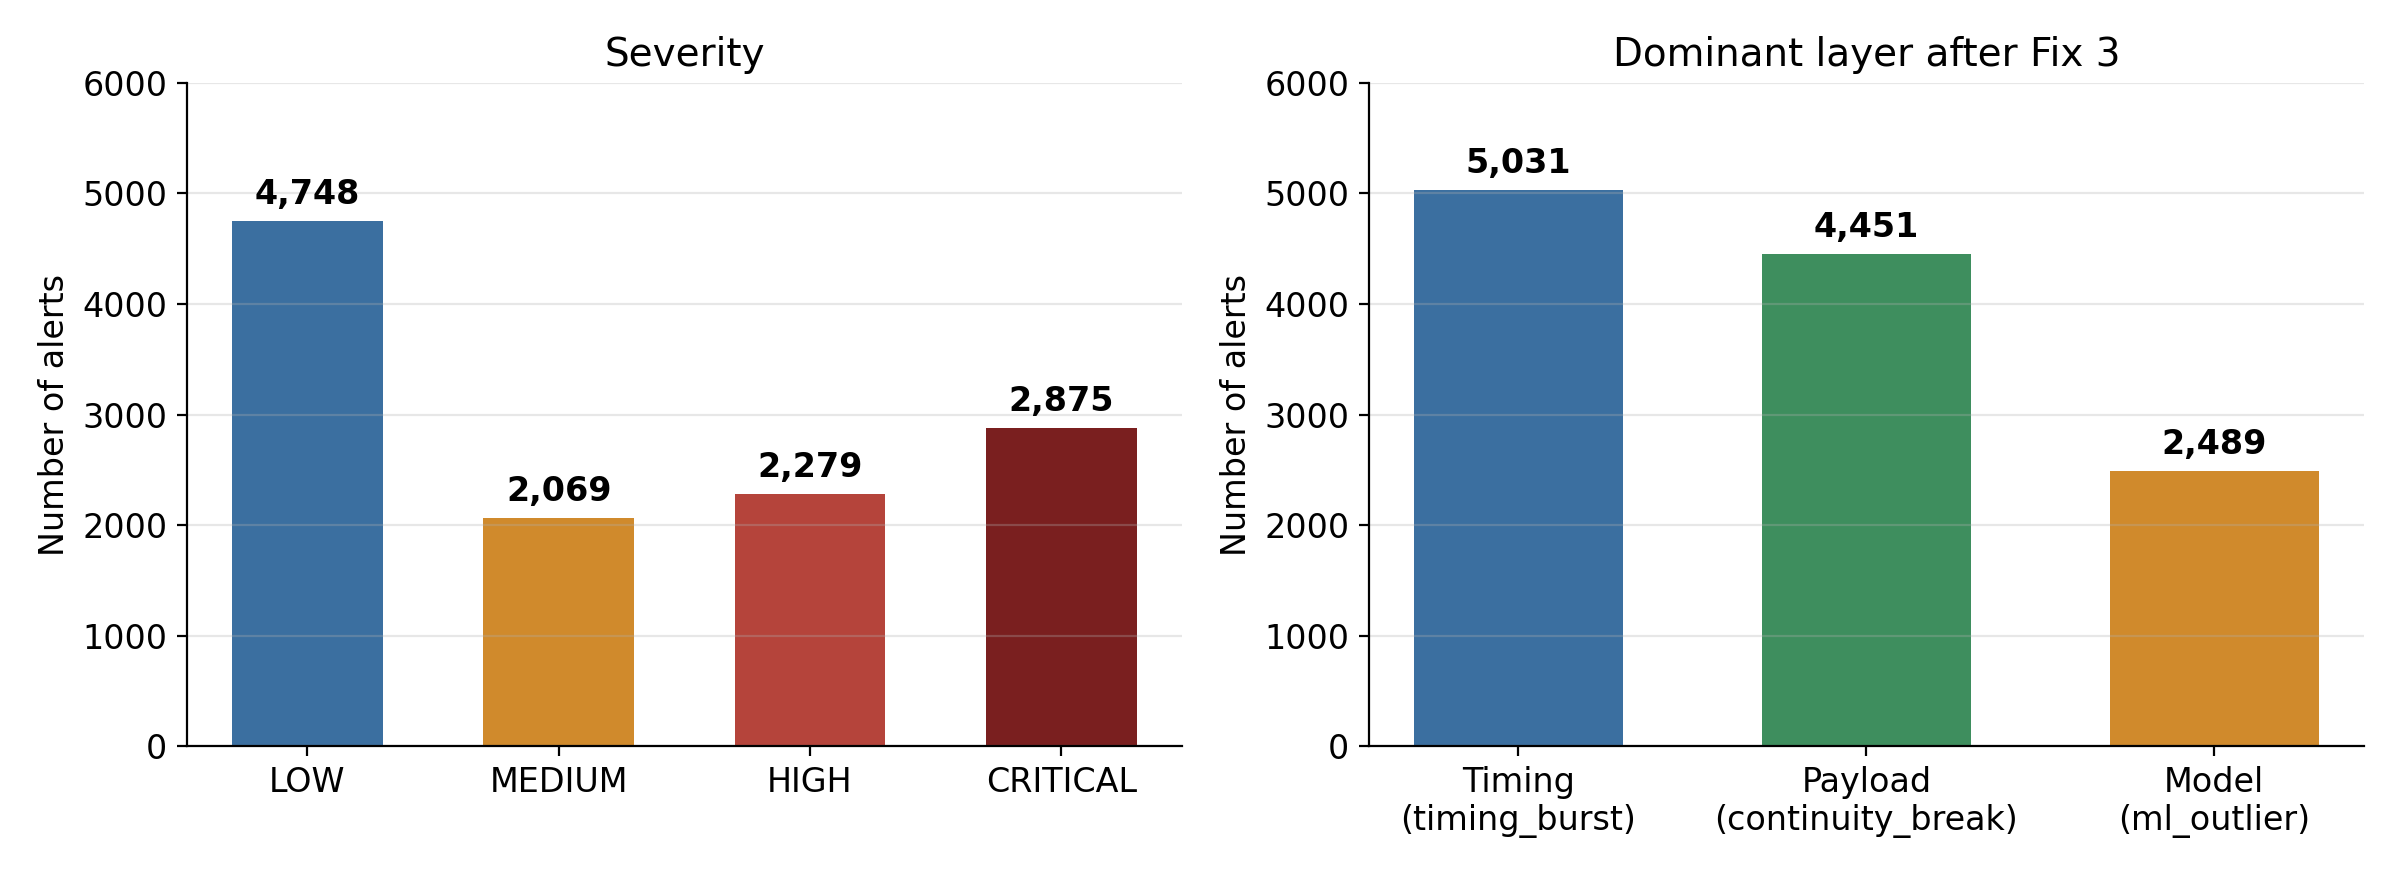
\includegraphics[width=\textwidth]{alert_breakdown.png}
\caption[Severity and dominant layer of the alerts after Fix 3.]{Severity (left) and dominant layer after Fix 3 (right) of the 11,971 alerts produced by the corrected first pipeline.}
\label{fig:chart-severity}
\end{figure}

\subsection{Assessment}

Table~\ref{tab:fixes-summary} summarises the six defects.

\begin{table}[H]
\centering
\small
\caption{Defects corrected during the second iteration.}
\label{tab:fixes-summary}
\begin{tabularx}{\textwidth}{|l|Y|c|}
\hline
\textbf{\#} & \textbf{Defect} & \textbf{Status} \\
\hline
1 & Vehicle model never used for scoring & Fixed, verified \\
\hline
2 & Driving state always classified as ``parking'' & Fixed, verified \\
\hline
3 & Diagnostic fields dominating the displayed cause (6 places) & Fixed, verified \\
\hline
4 & Replay formats other than \gls{csv} bypassing the common parser & Fixed, verified \\
\hline
5 & Polling timer left stopped after an import & Fixed, verified \\
\hline
6 & Explanation cache returning data from another session & Fixed, verified (two changes) \\
\hline
\end{tabularx}
\end{table}

All six defects were silent: none crashed or raised an error, and each appeared only when what the system reported was compared with a fact known independently, such as a vehicle being driven or a file being valid. The corrections reduced the alerts by a quarter without touching the threshold. The corrected pipeline worked, but the iteration exposed three weaknesses of its design. Two models in a chain meant that a wrong state selected the wrong forest, the source of two of the six defects. One forest per state mixed identifiers sent every 10 milliseconds with identifiers sent every second. And the fallbacks hid missing models. It was also not always possible to prove which data and settings had produced a model file. These weaknesses led to the rebuild of the models, planned as the fourth iteration, after the hardware milestone.

% ============================================================
\section{Iteration 3: hardware layer and bench rig}
\label{sec:it3}

\subsection{Objectives}

The third iteration delivered milestone M2: live capture from a physical \gls{can} adapter (FR9), and a way to test it without a vehicle, since none was available.

\subsection{Use cases addressed}

This iteration addressed the use case \emph{Connect hardware}, together with \emph{Detect anomaly}, applied to the frames of the live bus, and \emph{Record session}, which saves a live session to a log file.

\subsection{Design}
\label{sec:design-hardware}

The hardware layer wraps python-can, so it accepts the adapters python-can drives, such as slcan serial adapters, PEAK PCAN or SocketCAN, plus a virtual bus for tests. Every received frame goes to the same runtime engine as replay, built for the model chosen by the analyst, and is decoded with the \gls{dbc} file of the vehicle when it has a profile. A profile can declare its \gls{dbc} file complete, meaning that it defines every identifier of the bus, and live capture then flags any other identifier; since the \gls{dbc} files of real vehicles are partial, only a profile written for a known test bus can do so. Because the engine is shared, a bench rig test without a vehicle is meaningful for the part specific to live capture, its transport, while the engine behind it is the one that scores replays.

\subsection{Implementation}
\label{sec:impl-hardware}

Connecting an adapter builds a live engine for the model chosen by the analyst, and disconnecting stops the scoring. When no frame arrives for a few seconds, the link is reported as lost. Frames are decoded with the \gls{dbc} file of the selected profile and, with a complete profile, a frame on an identifier outside the file raises an alert on the whitelist layer.

Our bench rig replaces the vehicle. Two Arduino Uno boards, each with an MCP2515 \gls{can} module, are joined by a two wire bus terminated with 120\,$\Omega$ resistors, at 500~kbit/s. The bridge board is connected by USB and runs a small firmware that speaks the slcan protocol expected by python-can. The simulator board sends a speed frame every 20 milliseconds and a state of charge frame every 200 milliseconds, about 55 frames per second, and, from the 35th second after power on, a frame every twenty seconds on an identifier that should not exist (0x666), which the profile of the rig leaves out on purpose.

\subsection{Tests}
\label{sec:validation-bench}

Live capture was tested on the bench rig in two steps. First, a short script read the bus through python-can: the three identifiers arrived with the values of the firmware, a speed of 60~km/h and a state of charge of 78\%, which showed that both boards, the wiring and the serial link worked. Second, the rig was connected from the application (slcan, 500~kbit/s), so that the frames went through the hardware layer into the runtime engine.

This second step revealed two defects of the hardware layer, which we corrected:

\begin{itemize}
    \item \textbf{One bad line closed the session.} After about eight minutes and 16{,}304 frames received, a single malformed line on the serial link raised an error that ended the connection. One bad frame does not mean that the link is dead, so the hardware layer now skips such a line, logs it and keeps reading. After this change, the connection stayed up and received frames at about 55 per second, the rate of the firmware.
    \item \textbf{Old data stayed on screen after the rig was unplugged.} When the boards were disconnected, the link was still reported as up, because its status only changed on a hard error, and the live screens kept showing the last frames received, hours later. The link is now reported as lost when no frame has arrived for five seconds, disconnecting clears the buffers of live data, and each live update says whether it comes from the hardware or from the simulator, so that the client can show which one the analyst is looking at.
\end{itemize}

Two more gaps concerned the interpretation of live frames. First, the frames were not decoded correctly. The rig had been connected under the profile of a real vehicle, whose \gls{dbc} file does not define 0x316 or 0x3F9, and the live signal panel read the frames with a signal map shared by all vehicles, which gave them the meaning of unrelated messages from another manufacturer. Second, the frame on the unknown identifier was never raised as an alert, and it could not have been: the whitelist of \Sref{sec:design-pipeline} belonged to the offline analysis, and live capture had no check of the identifiers at all. We corrected both. The rig now has its own vehicle profile and \gls{dbc} file, and the live screens use the decoding of the selected profile first, so the live values sent to the screens become a speed of 60~km/h and a state of charge of 78\%. The profile of the rig declares its \gls{dbc} file complete, so live capture flags 0x666 on its first frame, without any learning window. Automated tests send the three frames of the rig through the virtual bus of python-can and check the decoded values, the alert on 0x666, and the absence of such alerts for a profile whose \gls{dbc} file is partial.

\subsection{Assessment}

The transport of live capture, from the bus to the runtime engine, works on the bench rig. This test does not measure detection: the traffic of the rig is synthetic and much simpler than the traffic of a vehicle. We have not yet repeated the run on the physical rig after the last corrections, and the test was made before the final models of the fourth iteration were promoted. Risk R1 remains open: live capture has not been tested on a vehicle.

% ============================================================
\section{Iteration 4: model rebuild}
\label{sec:it4}

\subsection{Objectives}

The fourth iteration rebuilt every vehicle model to remove the weaknesses found in the second iteration: one model per \gls{can} identifier instead of a chain of models, a record of how each model was built, and an evaluation on a complete recording kept out of training before any model enters production. It also measured the speed of the final models and compared Isolation Forest with the other candidate algorithms.

\subsection{Use cases addressed}

This iteration addressed the use cases \emph{Select vehicle} and \emph{Check model status}, since every model now has a status that decides what it may be used for, \emph{Detect anomaly} with the new models, and \emph{Describe capture}, which tells the analyst whether the selected model was trained or tested on the loaded file.

\subsection{Design}

\subsubsection{Final design: one model per CAN identifier}
\label{sec:impl-feature-eng}

In the final design, each vehicle has one Isolation Forest per \gls{can} identifier, with no driving state and no fallback: a frame is scored by the model of its identifier, or not at all.

\begin{itemize}
    \item \textbf{Features:} Nine features are computed over a short window of recent frames of the identifier: the time since the previous frame with its rolling mean and standard deviation, the byte difference with the previous frame with its rolling mean, standard deviation and maximum, the number of changed bytes, and the payload entropy. A feature that never changes for an identifier is dropped for it. The same code computes the features for training, offline analysis and live scoring.
    \item \textbf{Unscored frames:} An identifier needs 1{,}000 training rows to get a model; below that it is \emph{sparse}, an identifier whose features never vary is \emph{unmodelled}, and one absent from training is \emph{unseen}. Their frames, and the first frames of any identifier (\emph{warmup}), are reported as unresolved with their reason, so the analyst sees how much of a recording the models covered.
    \item \textbf{Threshold:} Each model has its own threshold, set so that 2\% of its training rows are flagged. The raw score is mapped to a normalised score: 0 at the median of the training rows, 0.5 at the threshold, closer to 1 as the frame becomes more anomalous. The 2\% value was fixed before any test recording was scored and never changed afterwards.
\end{itemize}

\Needspace{162pt}% keep the text with its float
Table~\ref{tab:model-params} lists the parameters, also recorded in the manifest of every model.

\begin{table}[H]
\centering
\small
\caption{Parameters of the final models.}
\label{tab:model-params}
\begin{tabularx}{\textwidth}{|P{3.6cm}|Y|}
\hline
Forest & scikit-learn Isolation Forest, 200 trees, random seed 42, no feature scaling (a tree splits on one feature at a time) \\
\hline
Window and warmup & The last 10 frames of the identifier; its first 10 frames are not scored \\
\hline
Minimum data & 1{,}000 training rows per identifier \\
\hline
Threshold & With $n$ training rows and $k = \lfloor 0.02\,n \rfloor$, the $(k+1)$th smallest raw score; a frame is flagged below it \\
\hline
\end{tabularx}
\end{table}

\subsubsection{Training and promotion pipeline}

Figure~\ref{fig:ml-training} shows how the models are produced. The corpus of each vehicle is split by recording, not by frame: at least one complete recording is kept aside as a \emph{holdout}, never used to fit the model or set its threshold, because two frames of the same recording are too similar for a frame level split to say anything about a new recording. The SHA-256 fingerprint of each file guarantees that no recording is used on both sides.

A training run writes the models into a staging folder with a \emph{manifest} that records the code versions, the Git commit, the parameters, the threshold, median and row count of each identifier, and the SHA-256 fingerprints of the model file and of every recording. When the backend loads a vehicle, it checks that the model file and the manifest agree and that no recording is on both sides, and refuses the model otherwise. After the holdout evaluation, the promotion step copies accepted models to production and archives the previous files.

\begin{figure}[H]
\centering
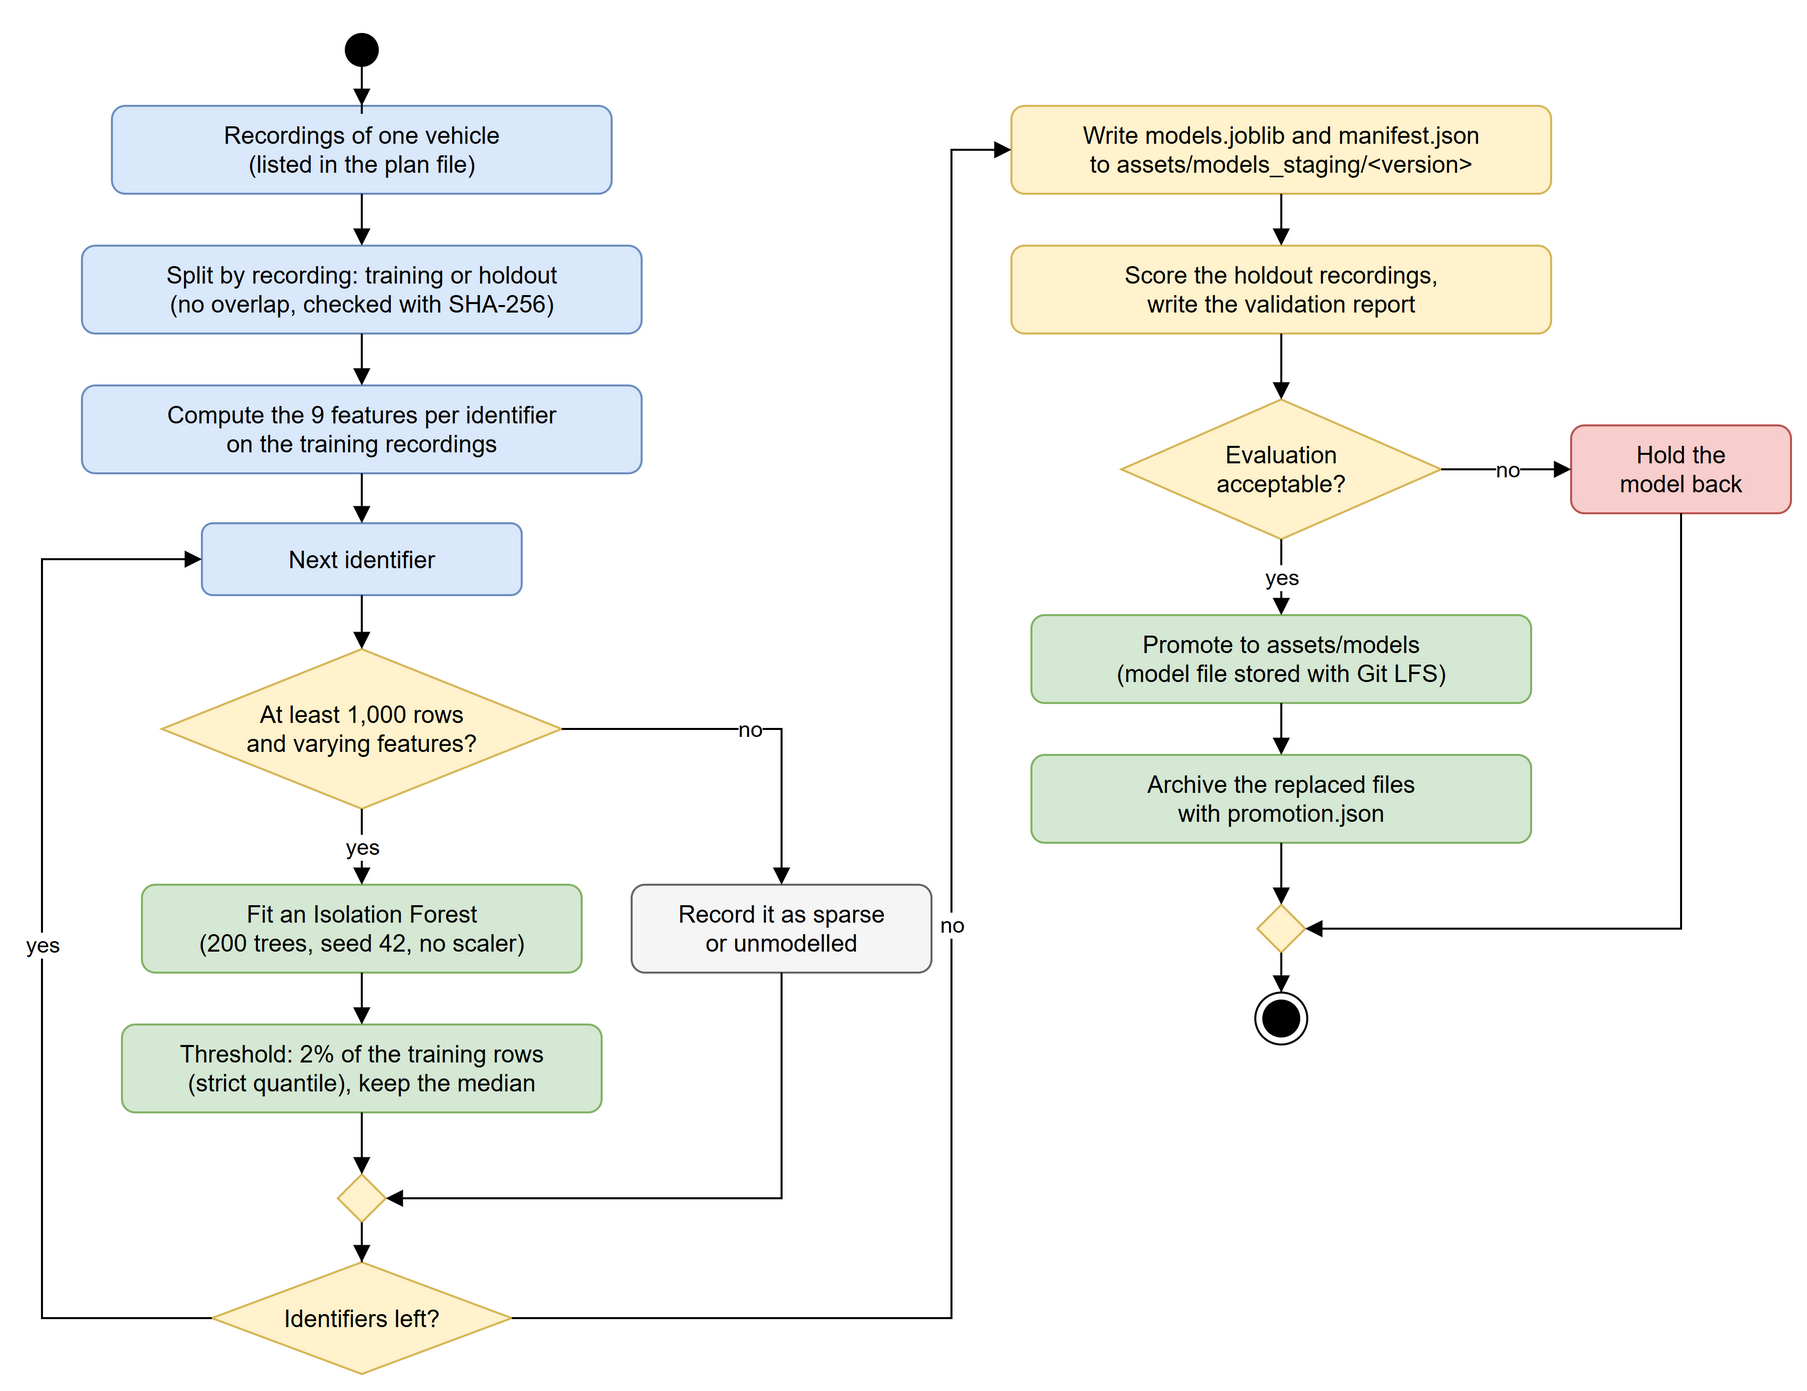
\includegraphics[width=\textwidth]{ml_training_pipeline.png}
\caption{Training pipeline, from the recordings of a vehicle to a model in production.}
\label{fig:ml-training}
\end{figure}

\Needspace{347pt}% keep the text with its float
\Needspace{133pt}% keep the heading with its float
\subsubsection{Model status}

Some vehicles have a single recording, so no holdout exists, and some models fail their evaluation. Each model therefore has a status that decides what it may be used for (Table~\ref{tab:model-status}), and the client shows it next to each model. Figure~\ref{fig:state-model-status} shows the life cycle of a model under the new pipeline as a state diagram.

\begin{table}[H]
\centering
\caption{Status of a model and what it allows.}
\label{tab:model-status}
\begin{tabularx}{\textwidth}{|P{4.6cm}|Y|}
\hline
\textbf{Status} & \textbf{Meaning and use} \\
\hline
Evaluated on a holdout & Final model in production. Used offline and live. \\
\hline
Not validated, no holdout & A final model exists, but the vehicle has only one recording. Refused offline; live capture uses the model of the first design, with a visible label. \\
\hline
Held back & Failed its evaluation. Refused offline and live. \\
\hline
No final model & No model could be built under the new rules. Refused. \\
\hline
Legacy & Only a model of the first design exists. Refused offline; accepted live with a visible label. \\
\hline
General & The general model of the first design, for a vehicle without its own model. \\
\hline
\end{tabularx}
\end{table}

\begin{figure}[H]
\centering
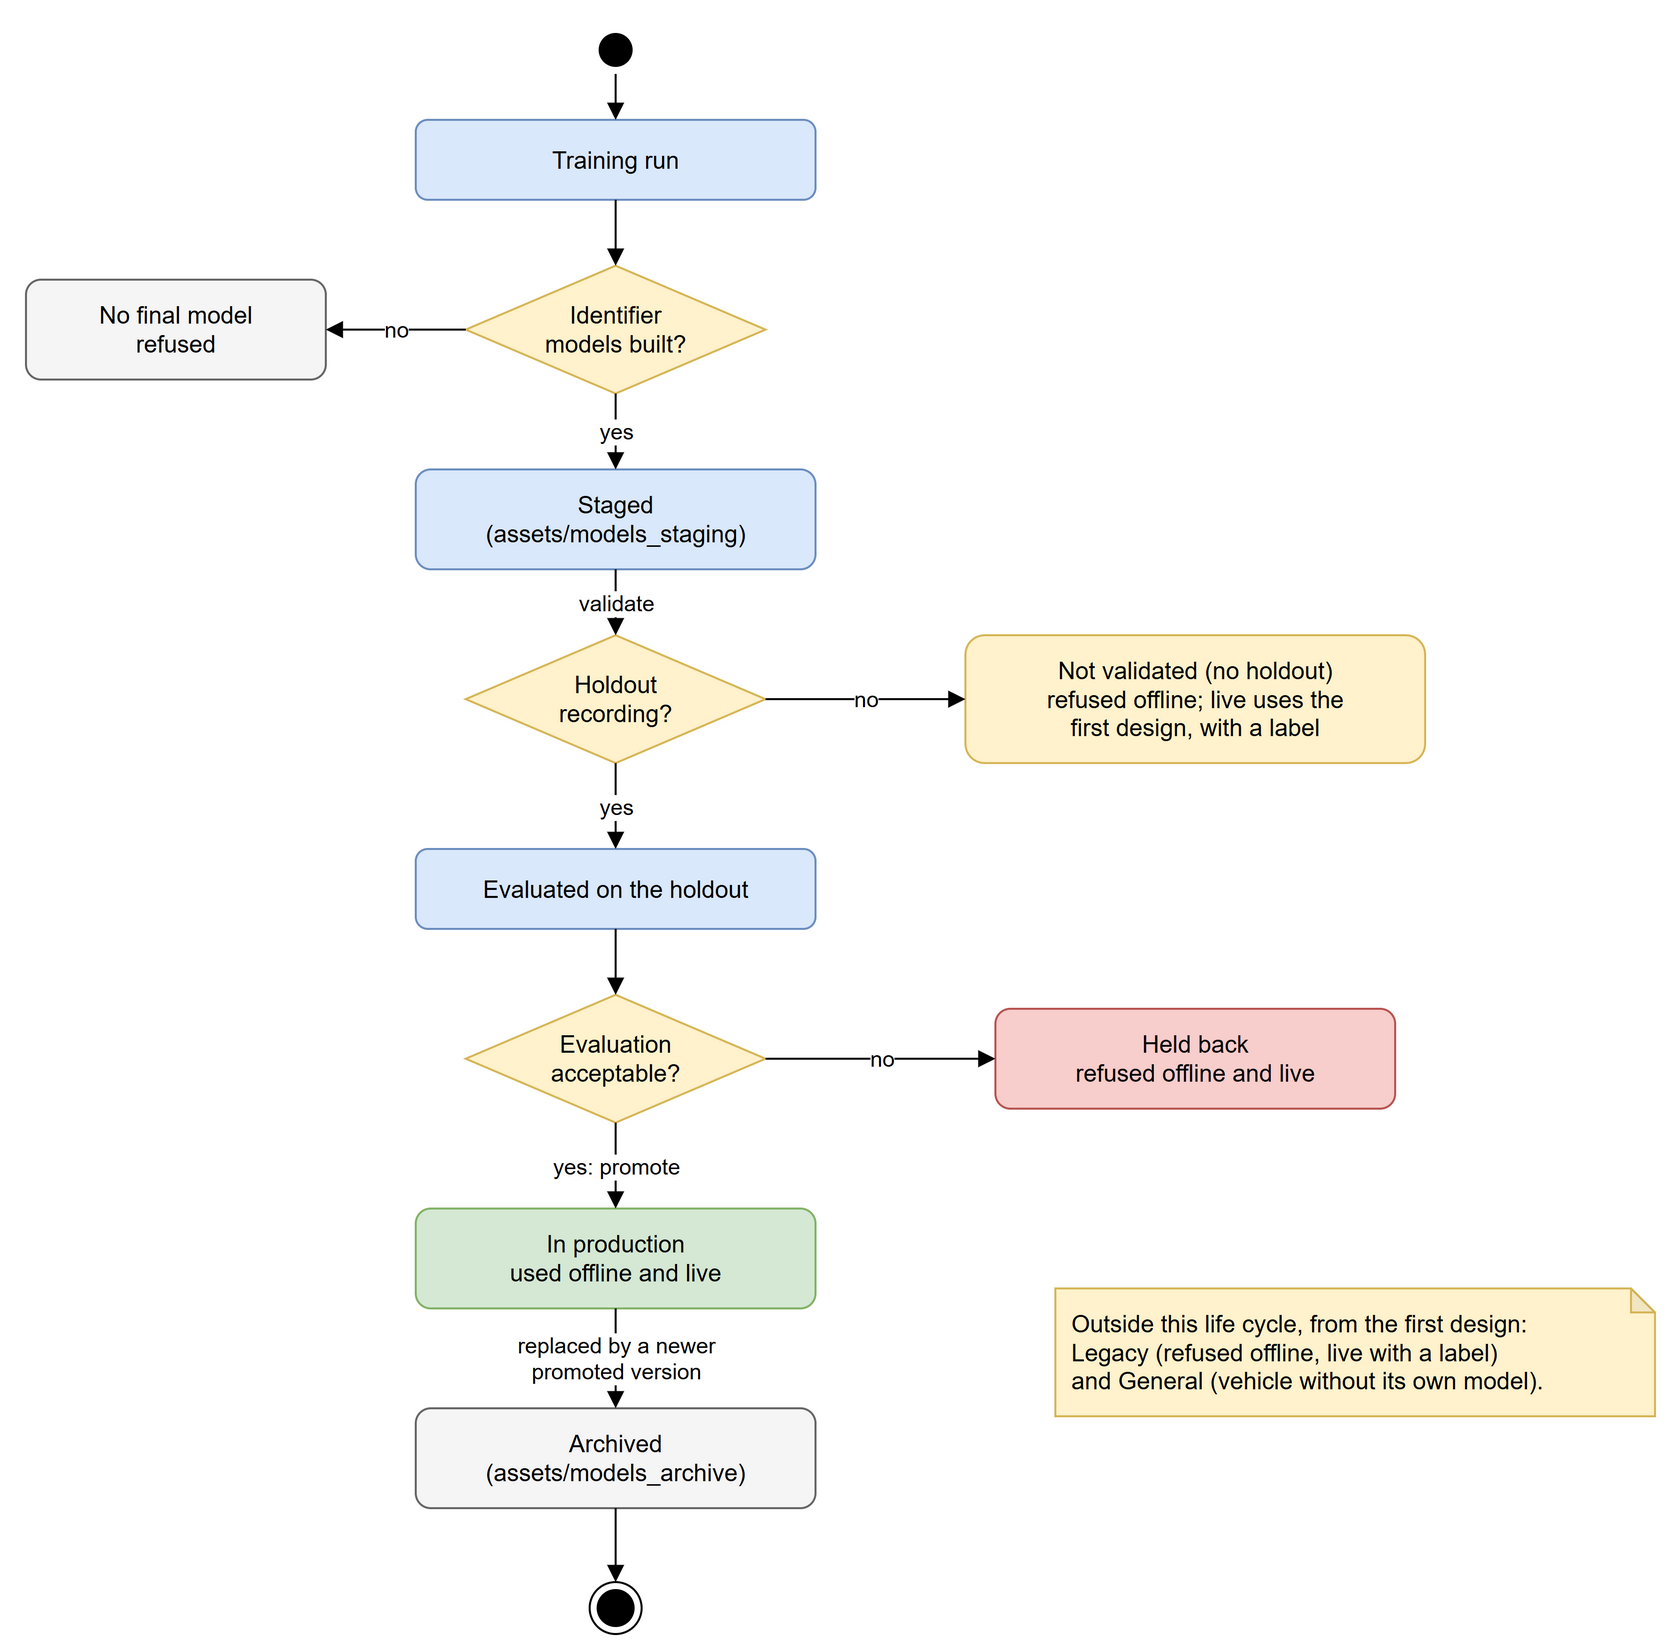
\includegraphics[height=0.62\textheight]{state_model_status.png}
\caption{State diagram: life cycle of a vehicle model.}
\label{fig:state-model-status}
\end{figure}

\subsection{Implementation}
\label{sec:impl-models}

The training pipeline is a set of Python scripts driven by a plan file that lists the training and holdout recordings of each vehicle. Its commands check the corpus and print the split without fitting anything, train a version into the staging folder, validate a staged version, and promote it. A run produces a validation report, read before any promotion; the promotion script refuses a held back vehicle and archives the files it replaces. The model files are stored with Git LFS.

At run time, one resolver gives the status of every model to the offline analysis, the live capture and the model list of the client, so they never disagree, and a model that may not be used is refused with an explicit reason instead of being replaced. The live engine of the hardware layer goes through the same resolver, so a held back or unknown model is refused for live capture too.

\label{sec:impl-capture}
The manifests also describe the recordings. The dataset card of the client sends the fingerprint of the loaded file to the backend, which looks it up in the manifest of the selected model and answers whether the model was trained on this file, tested on it, or never saw it. For the signals of a capture (FR12), the backend keeps the decoded signals that really change when a \gls{dbc} file exists, and ranks speed, state of charge, voltage, current and temperatures first; without one, it shows the raw payload bytes that change smoothly, as a physical value does, leaves out constants and rolling counters, and labels every raw channel as undecoded.

\subsection{Tests}

\subsubsection{Evaluation protocol}
\label{sec:validation-protocol}

Each final model was scored on every frame of its holdout recording, counting the frames scored, the frames flagged, and the frames that could not be scored, with their reason.

The holdout recordings carry no attack labels; we assume that they contain normal traffic but cannot prove it. We therefore report a \emph{flagged rate}, the share of scored frames that the model flagged, and not a false positive rate, a precision or a recall. If a holdout recording is entirely normal, every flagged frame in it is a false alarm and the flagged rate is the false alarm rate; if it is not, the flagged rate also contains real anomalies. Since each threshold flags 2\% of the training frames by construction, a flagged rate close to 2\% on a new recording means that the model sees this recording roughly as it saw its training data.

\subsubsection{Holdout results}

Table~\ref{tab:holdout-results} gives the results of the four models put into production. Together, they were trained on 23 recordings (3{,}436{,}061 frames) and evaluated on 1{,}130{,}500 frames of other recordings.

\begin{table}[H]
\centering
\footnotesize
\setlength{\tabcolsep}{4pt}
\caption{Final models scored on their holdout recordings.}
\label{tab:holdout-results}
\begin{tabular}{|l|r|r|r|r|r|r|}
\hline
\textbf{Vehicle} & \textbf{ID models} & \textbf{Training frames} & \textbf{Holdout frames} & \textbf{Scored} & \textbf{Flagged / scored} & \textbf{Rate} \\
\hline
Jaguar I-PACE & 46 & 233{,}598 & 50{,}361 & 82.6\% & 1{,}249 / 40{,}477 & 3.09\% \\
\hline
Kia EV6 & 161 & 448{,}198 & 438{,}170 & 98.4\% & 11{,}109 / 429{,}524 & 2.59\% \\
\hline
Nissan Leaf 2019 & 12 & 1{,}317{,}070 & 491{,}969 & 100.0\% & 2{,}951 / 491{,}797 & 0.60\% \\
\hline
ROAD ambient & 77 & 1{,}437{,}195 & 150{,}000 & 99.0\% & 8{,}982 / 147{,}485 & 6.09\% \\
\hline
\end{tabular}
\normalsize
\end{table}

The holdout recordings are \texttt{canbus\_turningon\_quickly.csv} for the Jaguar I-PACE, \texttt{Vehicle everthing on.asc} for the Kia EV6 (the spelling is the one of the original file), \texttt{00000001-61D9D9BA.MF4} for the Nissan Leaf 2019, and the first 150{,}000 frames of \texttt{ambient\_highway\_street\_driving\_long.log} for the ROAD vehicle. The \emph{Scored} column is the share of frames that belong to an identifier with a model, after warmup. The Jaguar I-PACE has the lowest coverage: on its holdout file, 8{,}451 frames belong to sparse identifiers, 1{,}368 are warmup frames and 65 belong to unseen identifiers, all reported as unresolved rather than normal.

We read these results as follows.

\begin{itemize}
    \item \textbf{Nissan Leaf 2019 (0.60\%).} The model flags fewer frames on its holdout than on its training data. The holdout comes from the same logger as the training recordings, and the model sees it as ordinary traffic.
    \item \textbf{Jaguar I-PACE (3.09\%) and Kia EV6 (2.59\%).} Both rates are close to the 2\% of the calibration, slightly above it, which is what we expected for a new session of the same vehicle.
    \item \textbf{ROAD ambient (6.09\%).} This rate is three times the calibration level. Most of the difference comes from one identifier, 0x193: its payload never changes in any training recording, but it does change on the highway recording used as holdout, and 58\% of its holdout frames are flagged. This is a difference of coverage between training and holdout, not a problem of threshold. We did not change the threshold after seeing the holdout, since this would have turned the holdout into training data.
\end{itemize}

\subsubsection{Models we did not put into production}

The same protocol showed which models not to trust. The MG ZS EV model flagged 43.60\% of the scored frames of its holdout, because about 78\% of its holdout frames belong to identifiers absent from its only training recording; it was held back. Three other model families (the Hyundai Ioniq 5, a Tesla and a Kaggle dataset of normal traffic) have a single recording, so their models are marked as not validated and refused by the offline analysis, and for two vehicles no final model could be built (Table~\ref{tab:model-status}).

\subsubsection{Consistency checks}

For every identifier model, the threshold recomputed from the training rows matched the manifest (rows, $k$, threshold, flagged rows and median), and the fingerprints confirmed that no recording is both in the training set and in the holdout of a vehicle.

\subsubsection{Speed of the final models}
\label{sec:validation-speed}

A benchmark replayed the first 10{,}000 frames of each holdout through the runtime engine, as live capture would (Table~\ref{tab:perf-live}).

\begin{table}[H]
\centering
\caption{Speed of the live path with the final models, on the first 10,000 frames of each holdout. The model call is given as mean and 99th percentile.}
\label{tab:perf-live}
\begin{tabular}{|l|>{\raggedleft\arraybackslash}p{2.2cm}|>{\raggedleft\arraybackslash}p{2.4cm}|>{\raggedleft\arraybackslash}p{2cm}|>{\raggedleft\arraybackslash}p{2.2cm}|}
\hline
\textbf{Vehicle} & \textbf{Bus (frames/s)} & \textbf{Processed (frames/s)} & \textbf{Real time factor} & \textbf{Model call (ms)} \\
\hline
Jaguar I-PACE & 2{,}990 & 262 & 0.09 & 23.6 / 32.7 \\
\hline
Kia EV6 & 448 & 224 & 0.50 & 23.5 / 33.8 \\
\hline
Nissan Leaf 2019 & 98 & 205 & 2.10 & 23.8 / 34.6 \\
\hline
ROAD ambient & 2{,}391 & 219 & 0.09 & 23.7 / 34.7 \\
\hline
\end{tabular}
\end{table}

One model call costs about 24 milliseconds, so even with the model called on every fifth frame, the live path processes about 200 to 260 frames per second. It keeps up with the Nissan Leaf (about 100 frames per second) but not with the Jaguar I-PACE or the ROAD vehicle (thousands per second), and reaches half of the Kia EV6 rate. The offline analysis scores whole batches: the 491{,}969 frames of the Leaf holdout took 187 seconds, and the Jaguar file 16 seconds in the backend and about one minute in the application. NFR1 is therefore met offline, and live only for slow buses.

\Needspace{396pt}% keep the heading with its float
\subsubsection{Comparison with the other candidate algorithms}
\label{sec:validation-compare}

As planned in \Sref{sec:ml-selection}, we measured LOF and the One Class SVM against Isolation Forest under the same conditions (Figure~\ref{fig:ml-compare-pipeline}). The four vehicles with a final model keep their production split, and every identifier with a final model is fitted three times, on the same features and the same training rows: at most 5{,}000 evenly spaced rows per identifier, because the One Class SVM does not scale to the largest ones. The three models get the threshold rule of the final models and score the holdout recording, which none of them saw.

\begin{figure}[H]
\centering
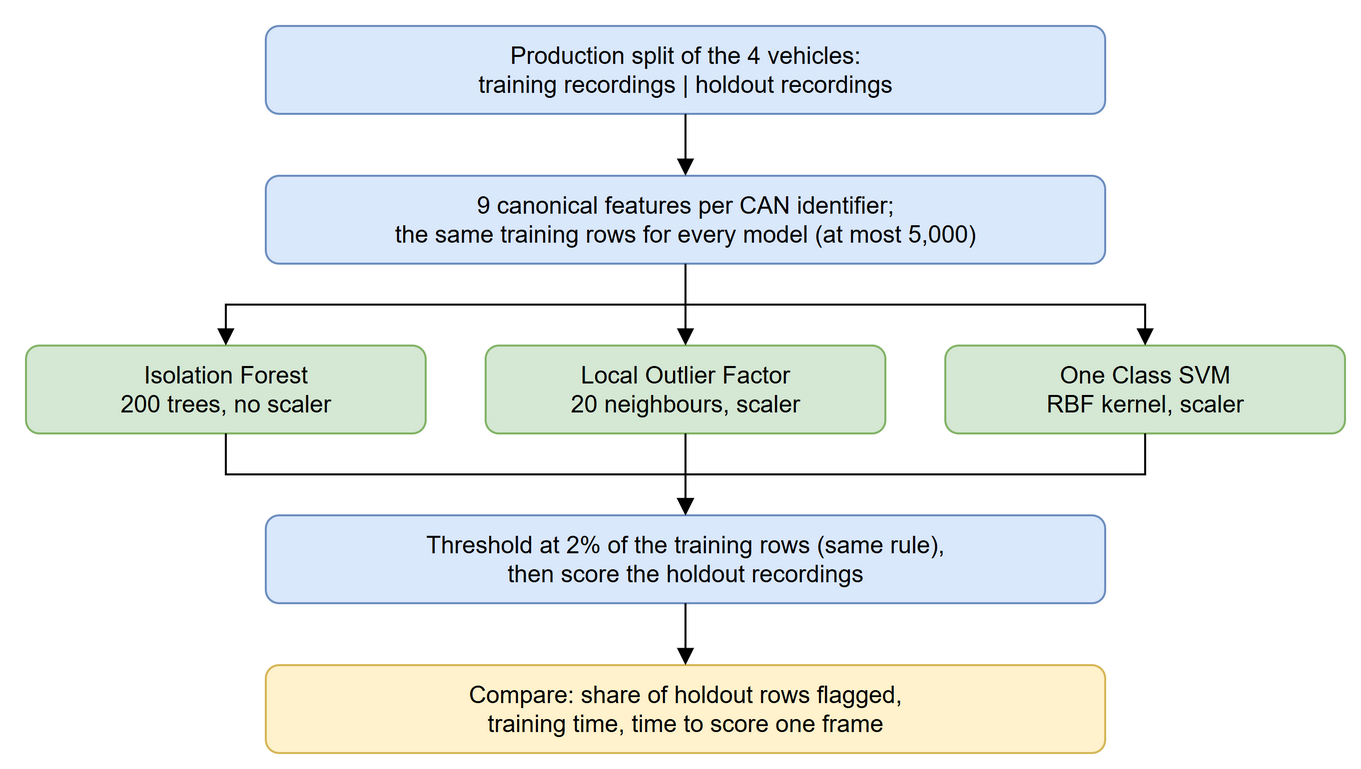
\includegraphics[width=0.8\textwidth]{ml_comparison_pipeline.png}
\caption[Pipeline of the algorithm comparison.]{Pipeline of the comparison: the same split, features, training rows and threshold rule for the three algorithms.}
\label{fig:ml-compare-pipeline}
\end{figure}

There are no attack labels, so the measure comes from the holdout recordings, which we assume to be normal traffic (\Sref{sec:validation-protocol}): every flagged row is then a false alarm, and a model whose boundary generalises flags about the 2\% of its calibration. Isolation Forest flags the fewest normal rows on average, 3.2\% against 5.1\% for LOF and 6.5\% for the One Class SVM, and has the lowest worst case, 6.4\% on ROAD against 13.1\% and 14.0\% on the Jaguar I-PACE (Figure~\ref{fig:ml-compare-flagged}). It is not the best everywhere: LOF does as well on the Kia EV6 and better on ROAD. Trained on these capped rows, Isolation Forest stays close to the final models trained on all rows (Table~\ref{tab:holdout-results}).

\begin{figure}[H]
\centering
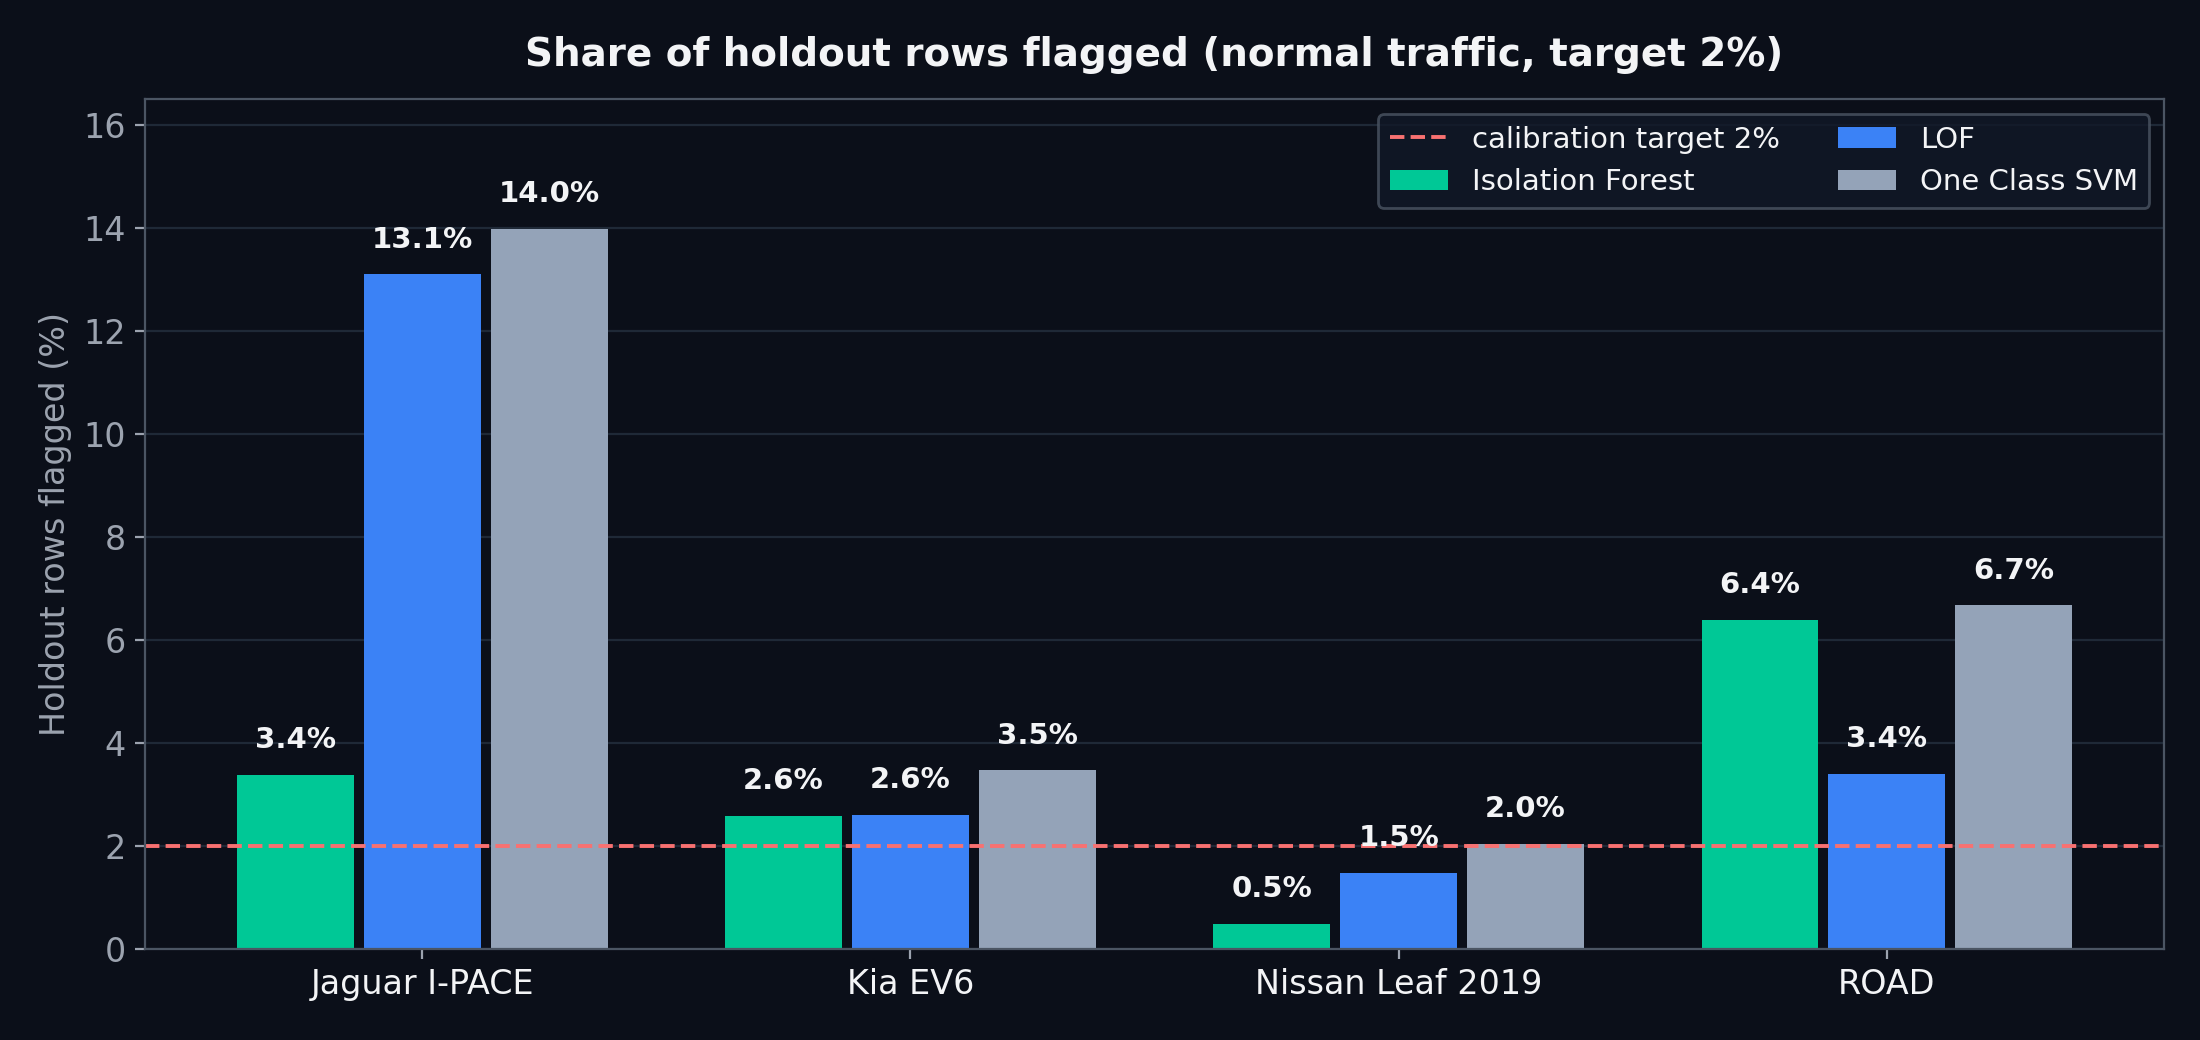
\includegraphics[width=\textwidth]{ml_compare_flagged.png}
\caption[Share of the holdout rows flagged by each algorithm.]{Share of the holdout rows flagged by each algorithm. The holdouts are assumed to be normal traffic, so a flagged row counts as a false alarm.}
\label{fig:ml-compare-flagged}
\end{figure}

This advantage has a price (Figure~\ref{fig:ml-compare-cost}). Isolation Forest is the slowest of the three: 138 seconds of training for the four vehicles against 41 and 17, and about 23 milliseconds to score one frame against 1 and 0.4. This is the model call measured in \Sref{sec:validation-speed}, and the reason the live path does not keep up with fast buses. We kept Isolation Forest because the offline analysis, the main use of the platform, needs few and even false alarms more than speed; LOF would score a live frame more than twenty times faster, at the cost of four times more false alarms on the Jaguar I-PACE.

\begin{figure}[H]
\centering
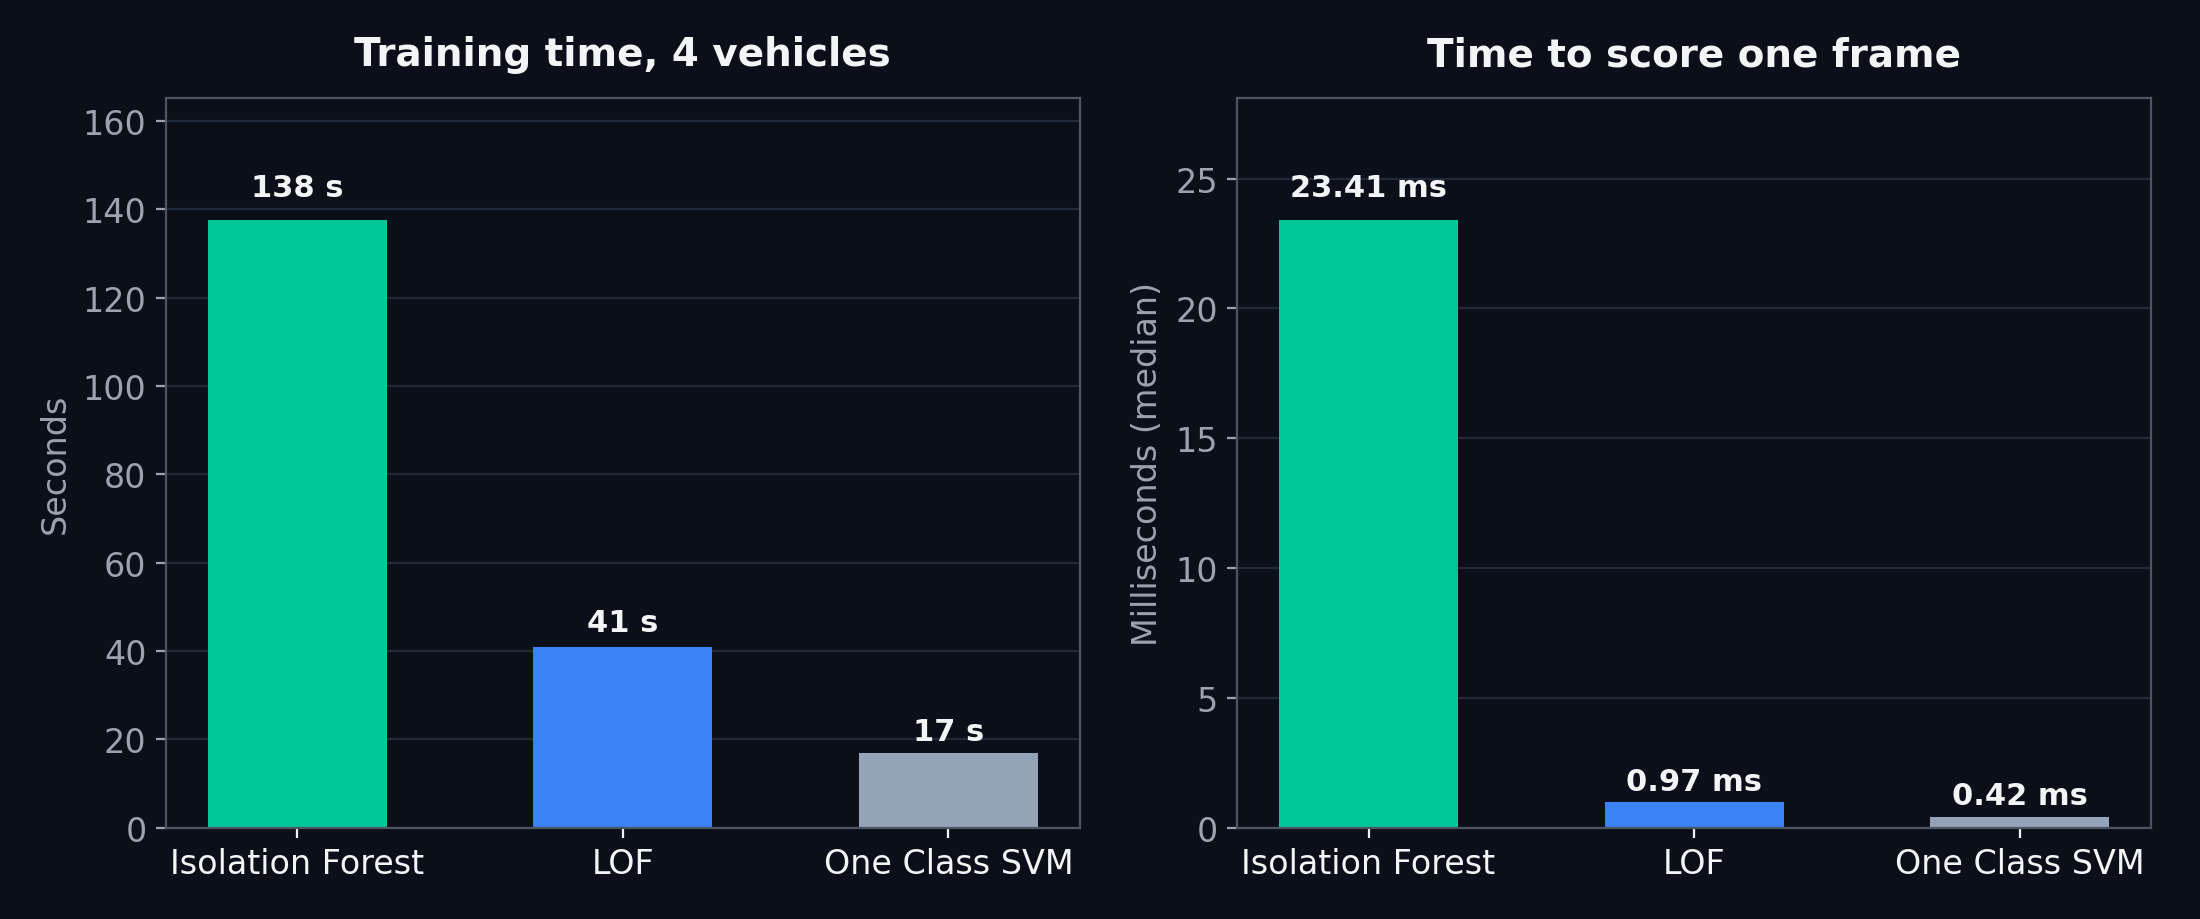
\includegraphics[width=\textwidth]{ml_compare_cost.png}
\caption[Training time and time to score one frame.]{Training time for the four vehicles, and median time to score one frame.}
\label{fig:ml-compare-cost}
\end{figure}

\Needspace{321pt}% keep the text with its float
Figure~\ref{fig:ml-feature-shares} shows what the final forests rely on. The three timing features carry about two thirds of the splits (64\%) and the six payload features the rest: for most identifiers, the sending rhythm is what isolates an unusual frame first.

\begin{figure}[H]
\centering
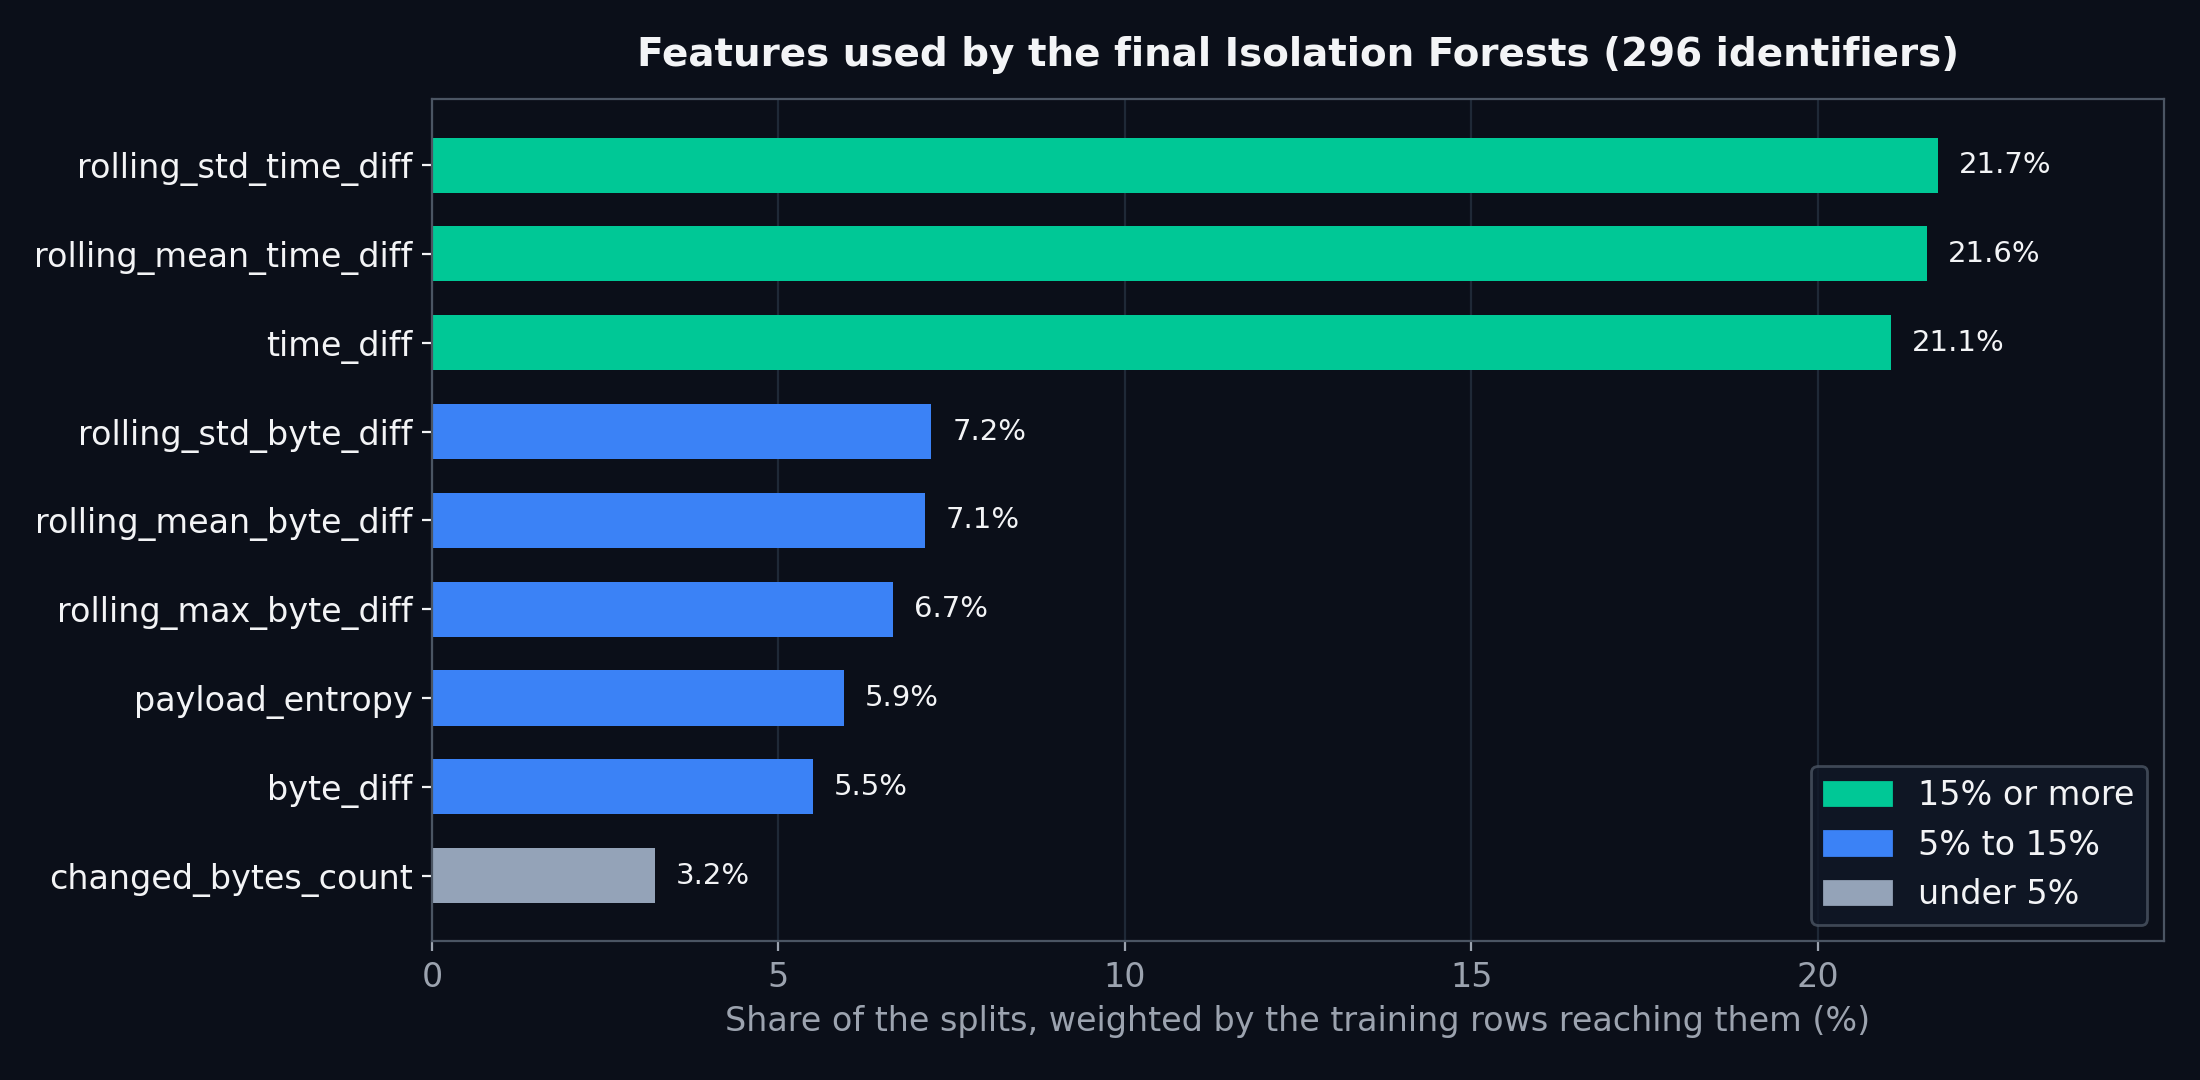
\includegraphics[width=\textwidth]{ml_feature_shares.png}
\caption[Features used by the final Isolation Forests.]{Features used by the final Isolation Forests: share of the splits, weighted by the training rows that reach them, averaged over the 296 identifier models.}
\label{fig:ml-feature-shares}
\end{figure}

\subsection{Assessment}

Four vehicles are in production, with 296 identifier models, each evaluated on a recording it never saw, with flagged rates from 0.60\% to 6.09\% that could each be explained. One model, the MG ZS EV, was held back because its evaluation showed that it could not be trusted. Isolation Forest was confirmed as the algorithm that flags the fewest normal rows, at the cost of a live path limited to slow buses.

\section*{Conclusion}
\addcontentsline{toc}{section}{Conclusion}

The four iterations of the construction phase delivered the first detection pipeline and the client, validated and corrected it on a real recording, added live capture tested on a bench rig, and rebuilt the models so that each one enters production only after an evaluation on unseen data. The next chapter presents the transition phase: the final release, its tests and its deployment.
